\documentclass[t,11pt,aspectratio=169]{beamer}
\usepackage{tikz}
\usepackage{pgfplots}
\usetikzlibrary{calc}
\usepackage[utf8]{inputenc}
\usepackage[ngerman]{babel}
\usepackage{amsmath,amsfonts,amssymb}
\usepackage{framed}
\usecolortheme{orchid}
\usepackage{etoolbox}
\useinnertheme[shadow=true]{rounded}

\usepackage{verbatim}

%%% PROGRESSBAR
\definecolor{pbblue}{HTML}{D8D8D8}% filling color for the progress bar
\definecolor{pbgray}{HTML}{F2F2F2}% background color for the progress bar
\useoutertheme{infolines}
\setbeamerfont{footline}{size=\normalsize}
\setbeamersize{text margin left=30pt,text margin right=30pt}
\makeatletter
\setbeamertemplate{footline}
{
	\leavevmode%
	\hbox{%
		\begin{beamercolorbox}[wd=.333333\paperwidth,ht=2.5ex,dp=1ex,center]{title in head/foot}%
			\usebeamerfont{title in head/foot}\insertshorttitle
		\end{beamercolorbox}%
		\begin{beamercolorbox}[wd=.333333\paperwidth,ht=2.5ex,dp=1ex,center]{date in head/foot}%
			%\usebeamerfont{date in head/foot}\insertshortdate{}\hspace*{2em}
			%\insertframenumber\hspace*{2ex} 
		\end{beamercolorbox}
		\begin{beamercolorbox}[wd=.333333\paperwidth,ht=3ex,dp=1ex,center]{author in head/foot}%
			\usebeamerfont{author in head/foot}\insertshortauthor~~%\beamer@ifempty{\insertshortinstitute}{}{(\insertshortinstitute)}
		\end{beamercolorbox}%
	}%
	\vskip0pt%
}
\makeatother
\makeatletter
\def\progressbar@progressbar{} % the progress bar
\newcount\progressbar@tmpcounta% auxiliary counter
\newcount\progressbar@tmpcountb% auxiliary counter
\newdimen\progressbar@pbht %progressbar height
\newdimen\progressbar@pbwd %progressbar width
\newdimen\progressbar@tmpdim % auxiliary dimension
\progressbar@pbwd=\linewidth
\progressbar@pbht=1.5ex
\def\progressbar@progressbar{%
    \progressbar@tmpcounta=\insertpagenumber
    \progressbar@tmpcountb=\insertdocumentendpage
    \progressbar@tmpdim=\progressbar@pbwd
    \multiply\progressbar@tmpdim by \progressbar@tmpcounta
    \divide\progressbar@tmpdim by \progressbar@tmpcountb
  \begin{tikzpicture}[rounded corners=3pt,very thin]
    \shade[top color=pbgray!20,bottom color=pbgray!20,middle color=pbgray!50]
      (0pt, 0pt) rectangle ++ (\progressbar@pbwd, \progressbar@pbht);
      \shade[draw=pbblue,top color=pbblue!50,bottom color=pbblue!50,middle color=pbblue] %
        (0pt, 0pt) rectangle ++ (\progressbar@tmpdim, \progressbar@pbht);
    \draw[color=normal text.fg!50]  
      (0pt, 0pt) rectangle (\progressbar@pbwd, \progressbar@pbht) 
        node[pos=0.5,color=normal text.fg] {\textnormal{%
             \pgfmathparse{\insertpagenumber*100/\insertdocumentendpage}%
             \pgfmathprintnumber[fixed,precision=0]{\pgfmathresult}\,\%%
        }%
    };
  \end{tikzpicture}%
}
\addtobeamertemplate{headline}{}
{%
  \begin{beamercolorbox}[wd=\paperwidth,ht=4ex,center,dp=1ex]{white}%
    \progressbar@progressbar%
  \end{beamercolorbox}%
}
\makeatother

\setbeamertemplate{frametitle}[default][center]

%%% BLOCKS
% block = Aufgabe
\setbeamercolor{block title}{fg=black,bg=blue!30!white} 
\setbeamercolor{block body}{fg=black, bg=blue!3!white}

% alertblock = Definition
\setbeamercolor{block title alerted}{fg=black,bg=red!50!white} 
\setbeamercolor{block body alerted}{fg=black, bg=red!3!white}

% exampleblock = Wiederholung
\setbeamercolor{block title example}{fg=black,bg=green!30!white} 
\setbeamercolor{block body example}{fg=black, bg=green!3!white}

\setbeamercovered{transparent}
\setbeamertemplate{navigation symbols}{}

\addtocounter{page}{-1}
\addtocounter{framenumber}{-1}
\setbeamercovered{invisible}





\begin{document}

\begin{frame}
Ausgangssituation:
$$ X_1,\dots,X_n\sim \mathcal{N}(\mu,\sigma^2)\text{~iid} $$
\pause

Folgende Hypothesen können wir testen:
\begin{itemize}
\item[a)] $H_0:\mu=\mu_0,~H_1:\mu\neq\mu_0$
\item[b)] $H_0:\mu\geq\mu_0,~H_1:\mu< \mu_0$
\item[c)] $H_0:\mu\leq\mu_0,~H_1:\mu > \mu_0$
\end{itemize}
\vspace{0.4cm}
\pause

Teststatistik:
$$ T=\frac{\bar{X}-\mu_0}{S}\sqrt{n},~\text{wobei}~S=\sqrt{\frac{1}{n-1}\sum_{i=1}^{n}(X_i-\bar{X})^2} $$
\pause

Verteilung der Teststatistik (für $\mu=\mu_0$):
$$T\sim t_{n-1}$$
\end{frame}

\begin{frame}
\begin{itemize}
\item[a)] $H_0:\mu=\mu_0,~H_1:\mu\neq\mu_0$ \hfill $T=\frac{\bar{X}-\mu_0}{S}\sqrt{n}\sim t_{n-1}$ \hfill
\end{itemize}
\begin{center}
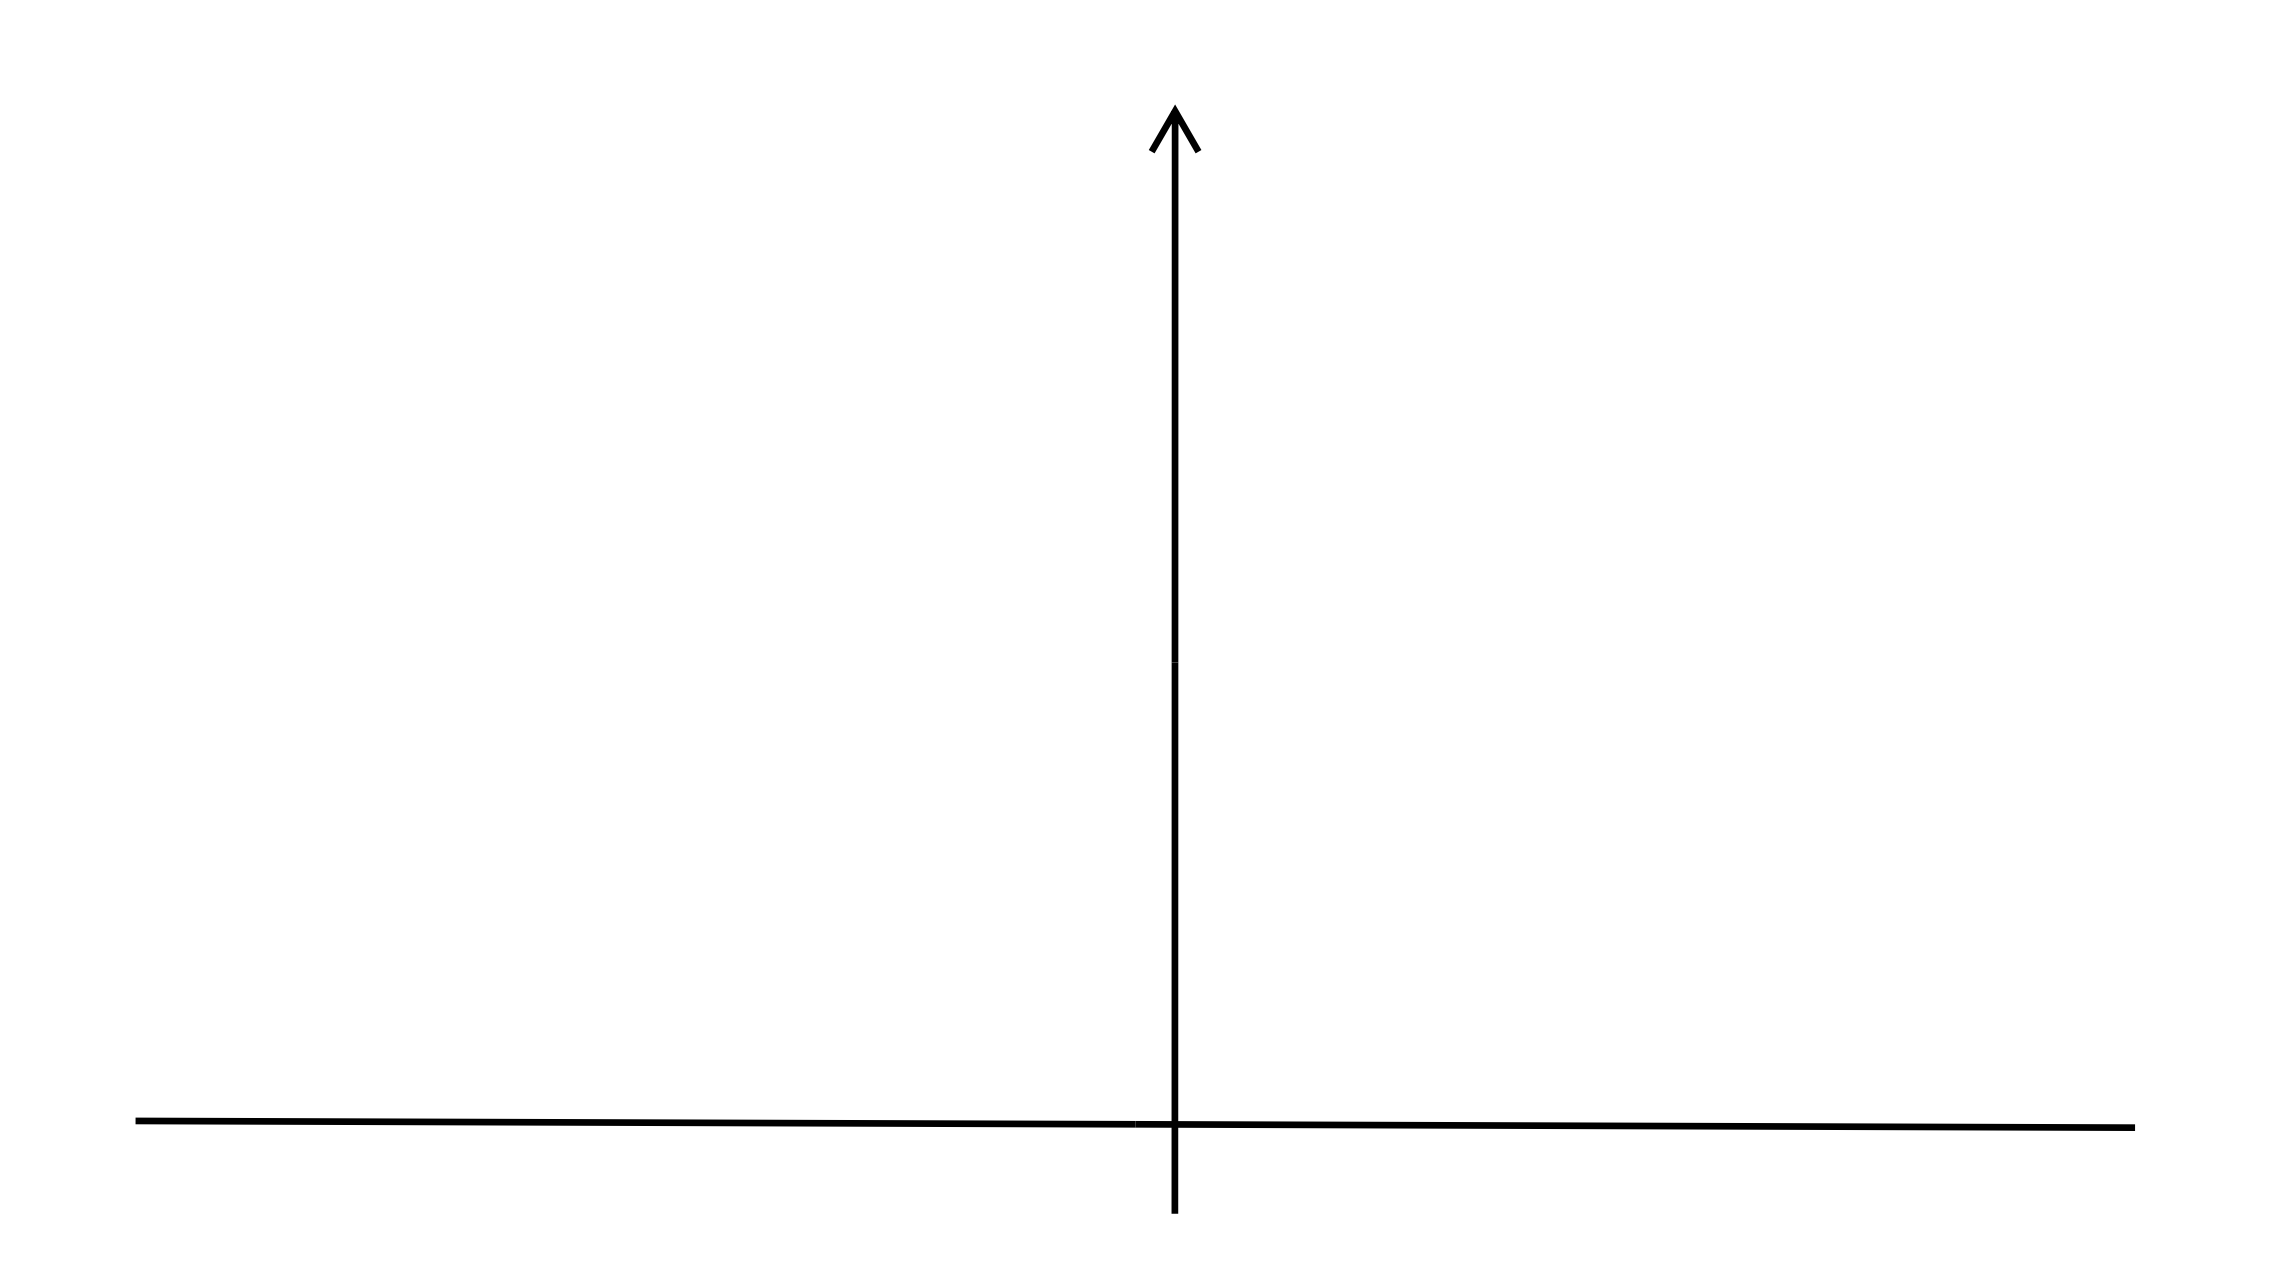
\includegraphics[scale=0.4]{1.png}
\end{center}
\end{frame}

\begin{frame}
\begin{itemize}
\item[a)] $H_0:\mu=\mu_0,~H_1:\mu\neq\mu_0$ \hfill $T=\frac{\bar{X}-\mu_0}{S}\sqrt{n}\sim t_{n-1}$ \hfill
\end{itemize}
\begin{center}
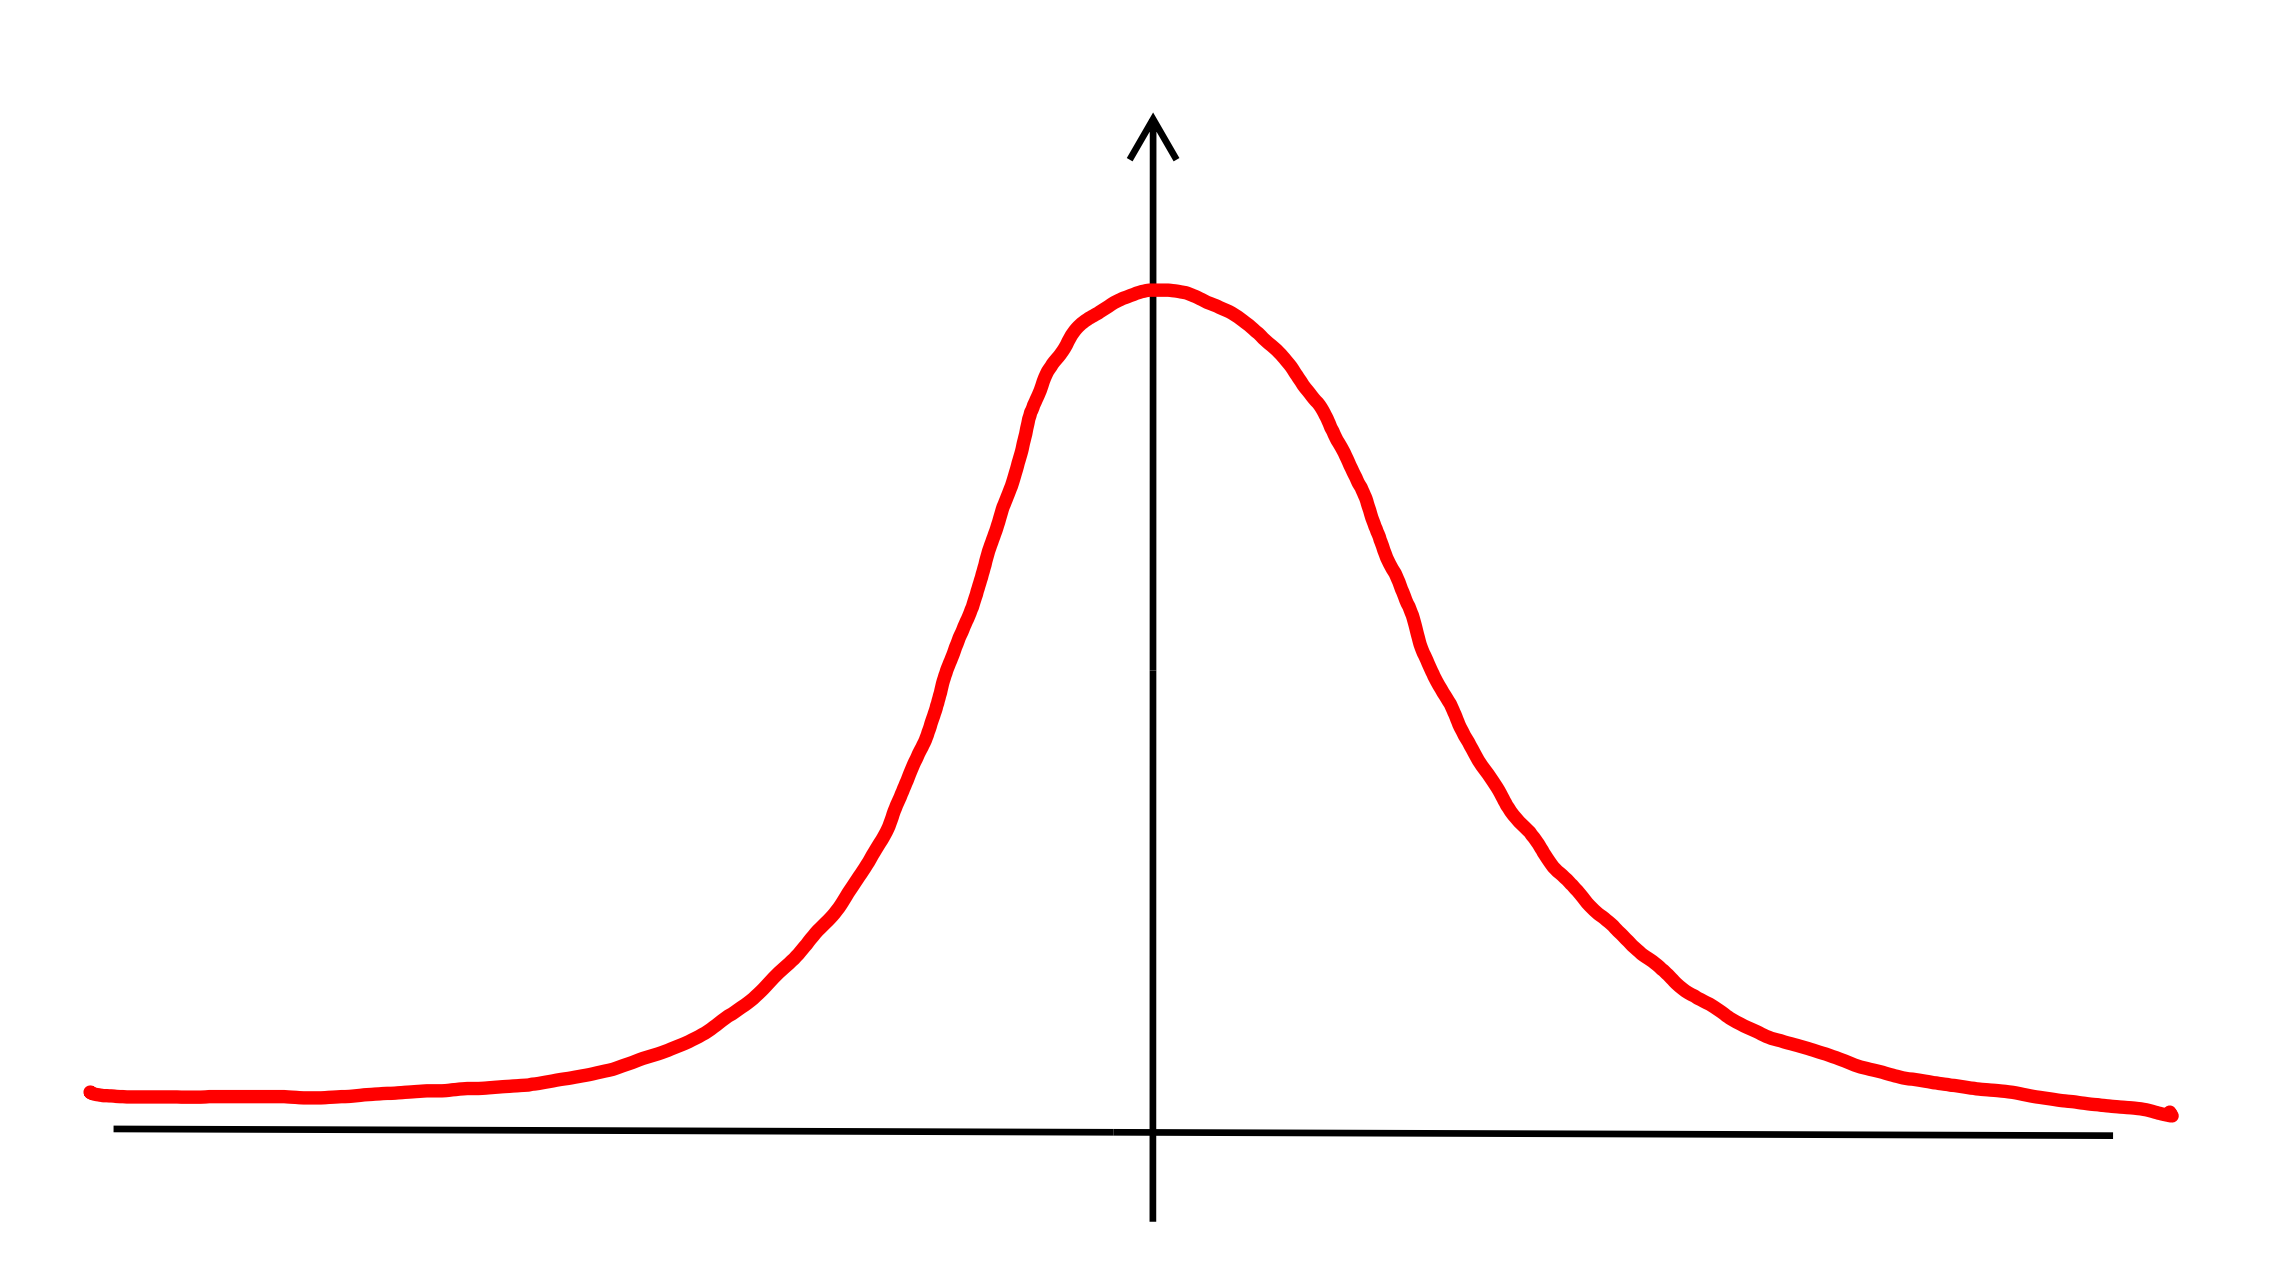
\includegraphics[scale=0.4]{2.png}
\end{center}
\end{frame}

\begin{frame}
\begin{itemize}
\item[a)] $H_0:\mu=\mu_0,~H_1:\mu\neq\mu_0$ \hfill $T=\frac{\bar{X}-\mu_0}{S}\sqrt{n}\sim t_{n-1}$ \hfill
\end{itemize}
\begin{center}
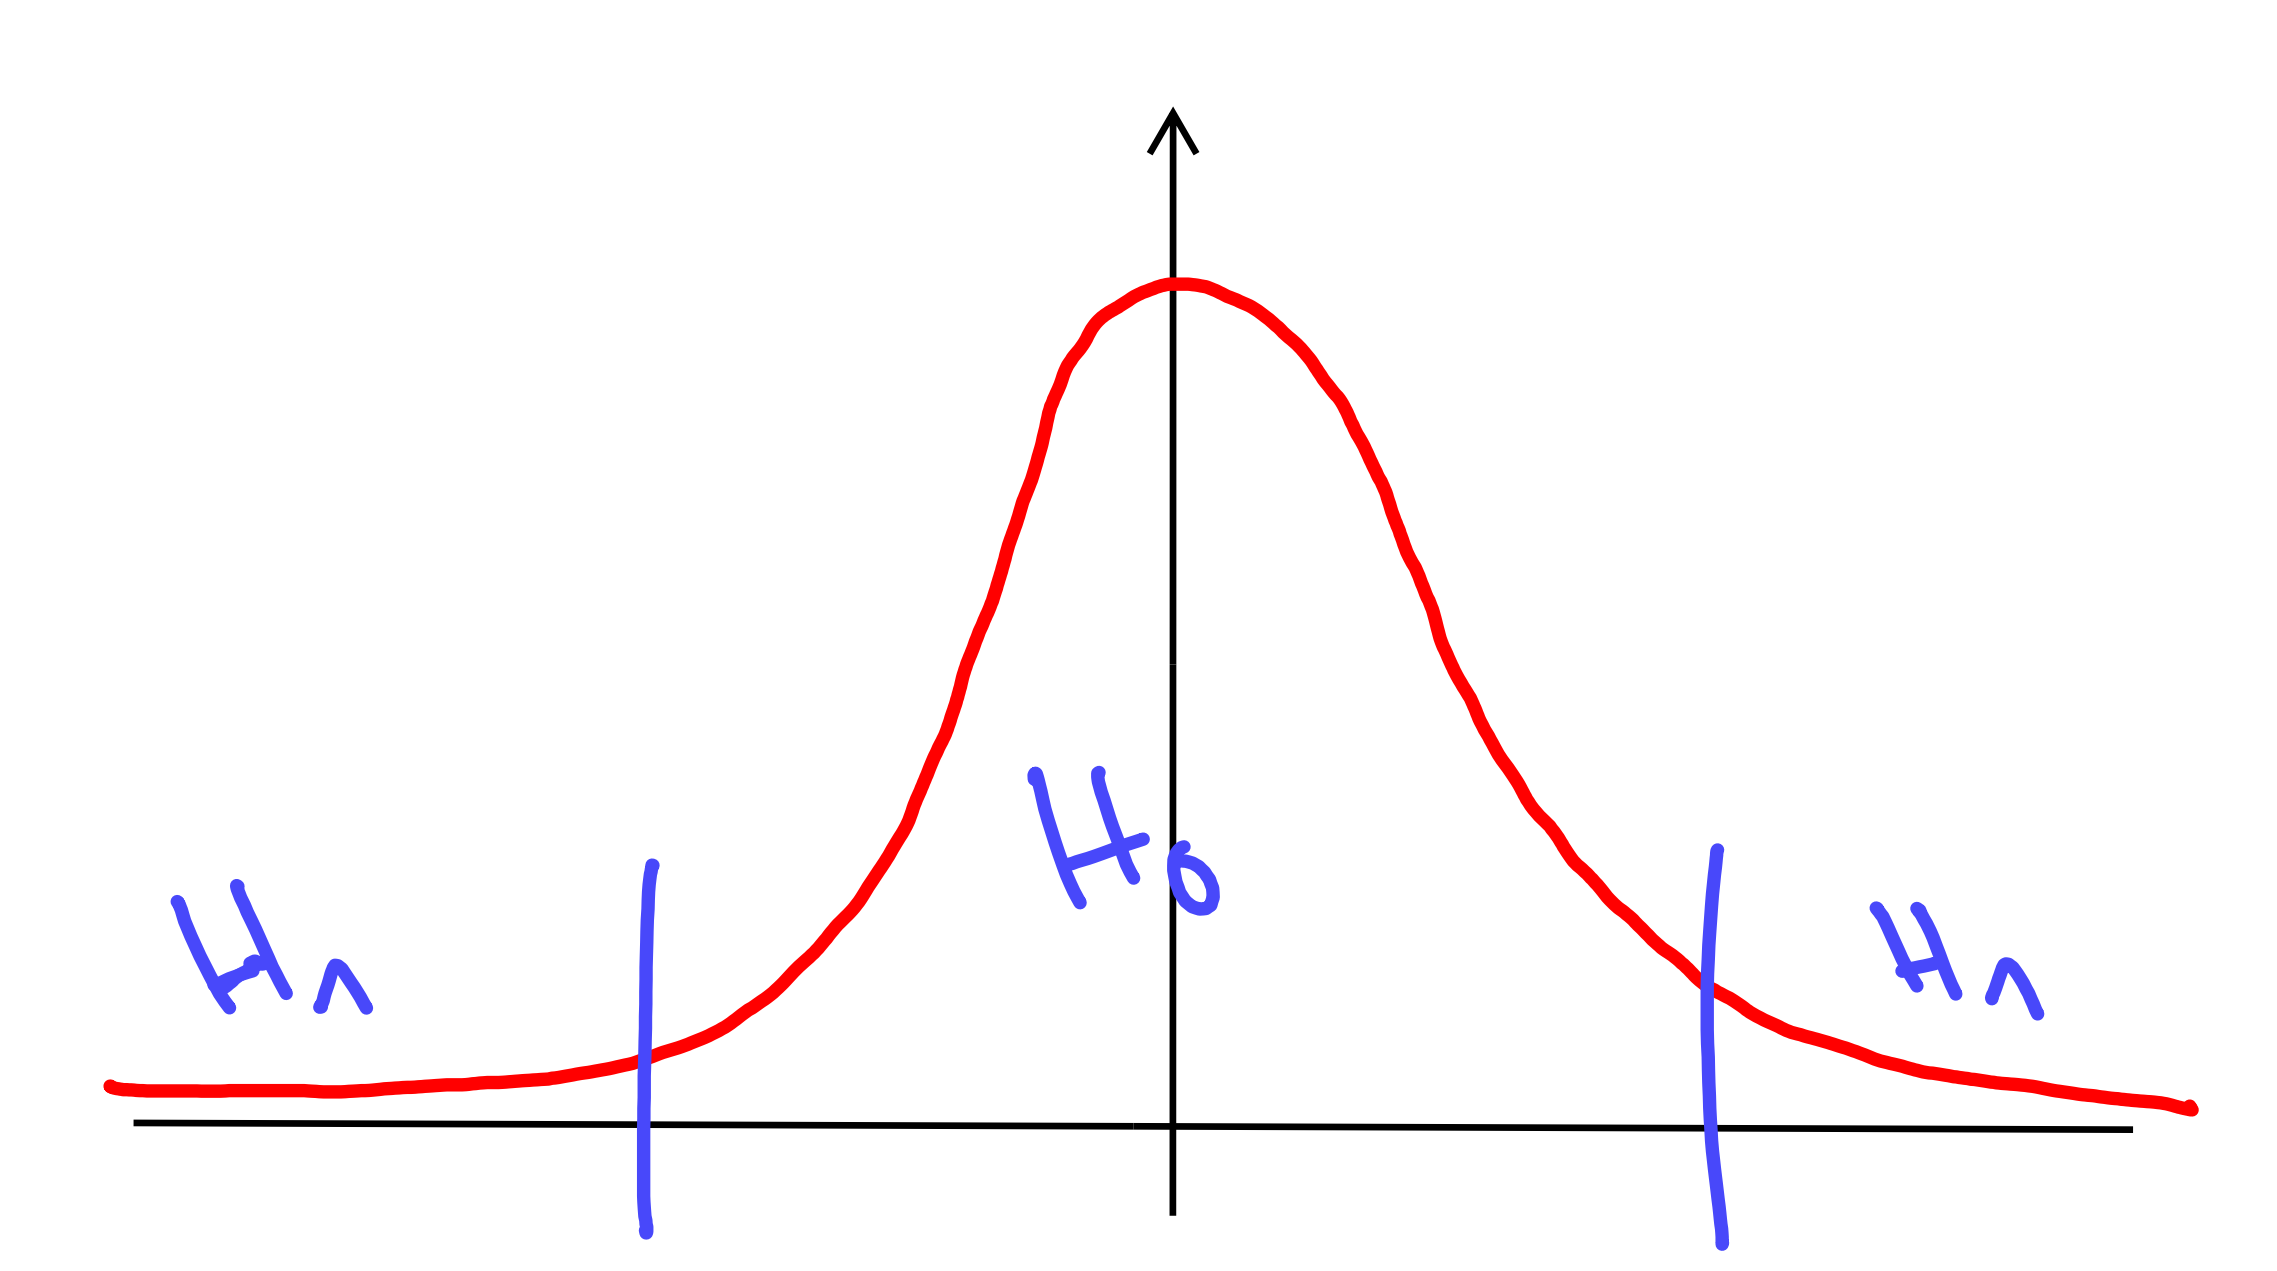
\includegraphics[scale=0.4]{3.png}
\end{center}
\end{frame}

\begin{frame}
\begin{itemize}
\item[a)] $H_0:\mu=\mu_0,~H_1:\mu\neq\mu_0$ \hfill $T=\frac{\bar{X}-\mu_0}{S}\sqrt{n}\sim t_{n-1}$ \hfill
\end{itemize}
\begin{center}
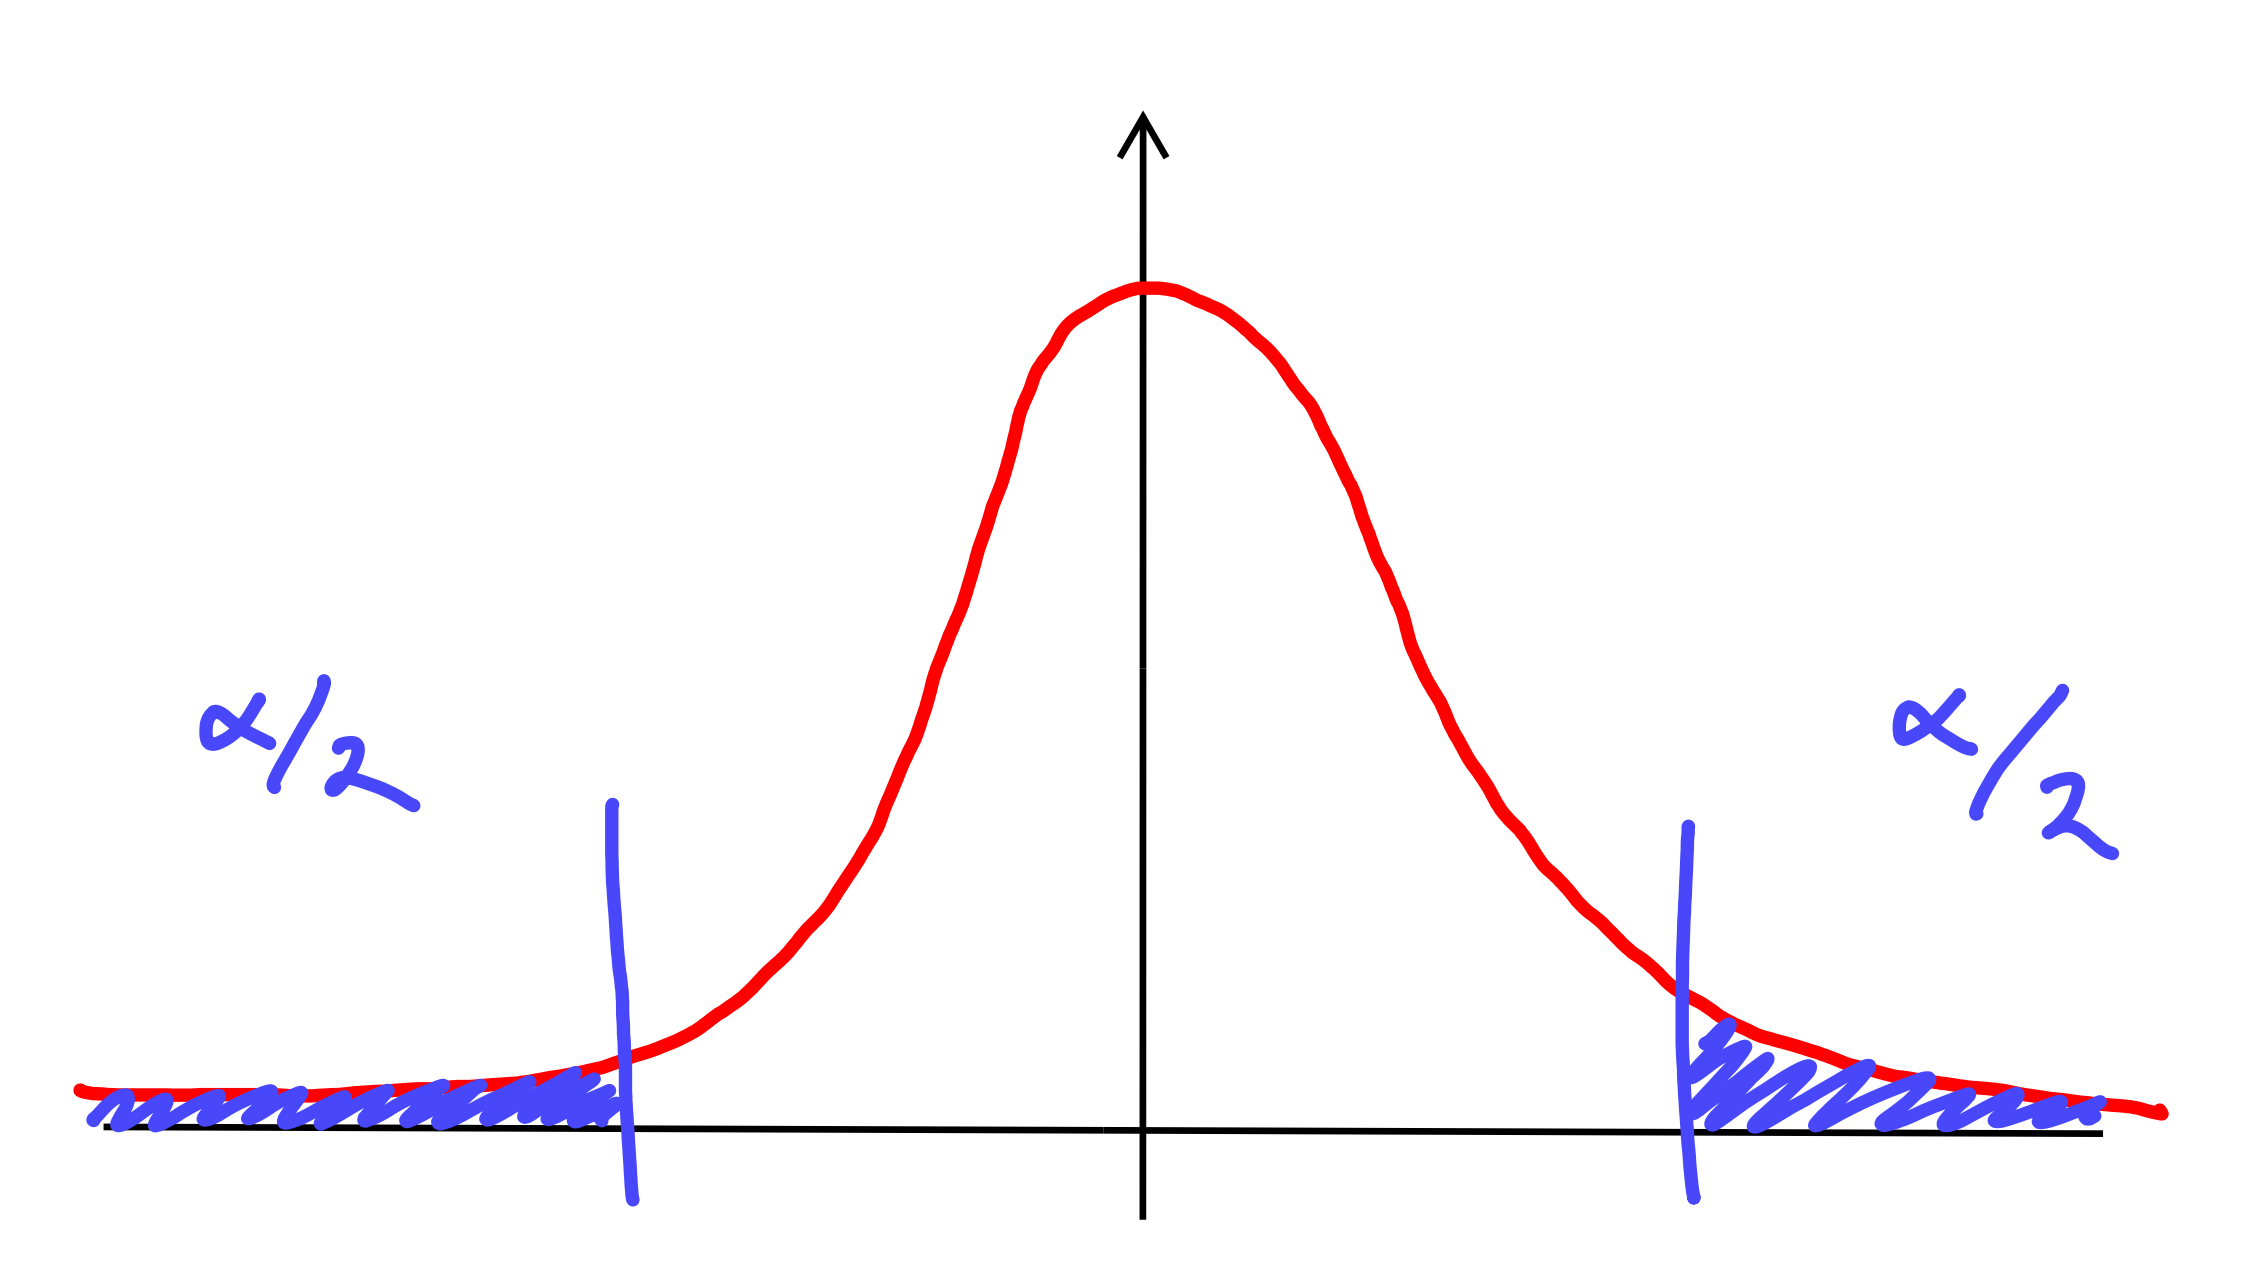
\includegraphics[scale=0.4]{4.png}
\end{center}
\end{frame}

\begin{frame}
\begin{itemize}
\item[a)] $H_0:\mu=\mu_0,~H_1:\mu\neq\mu_0$ \hfill $T=\frac{\bar{X}-\mu_0}{S}\sqrt{n}\sim t_{n-1}$ \hfill
\end{itemize}
\begin{center}
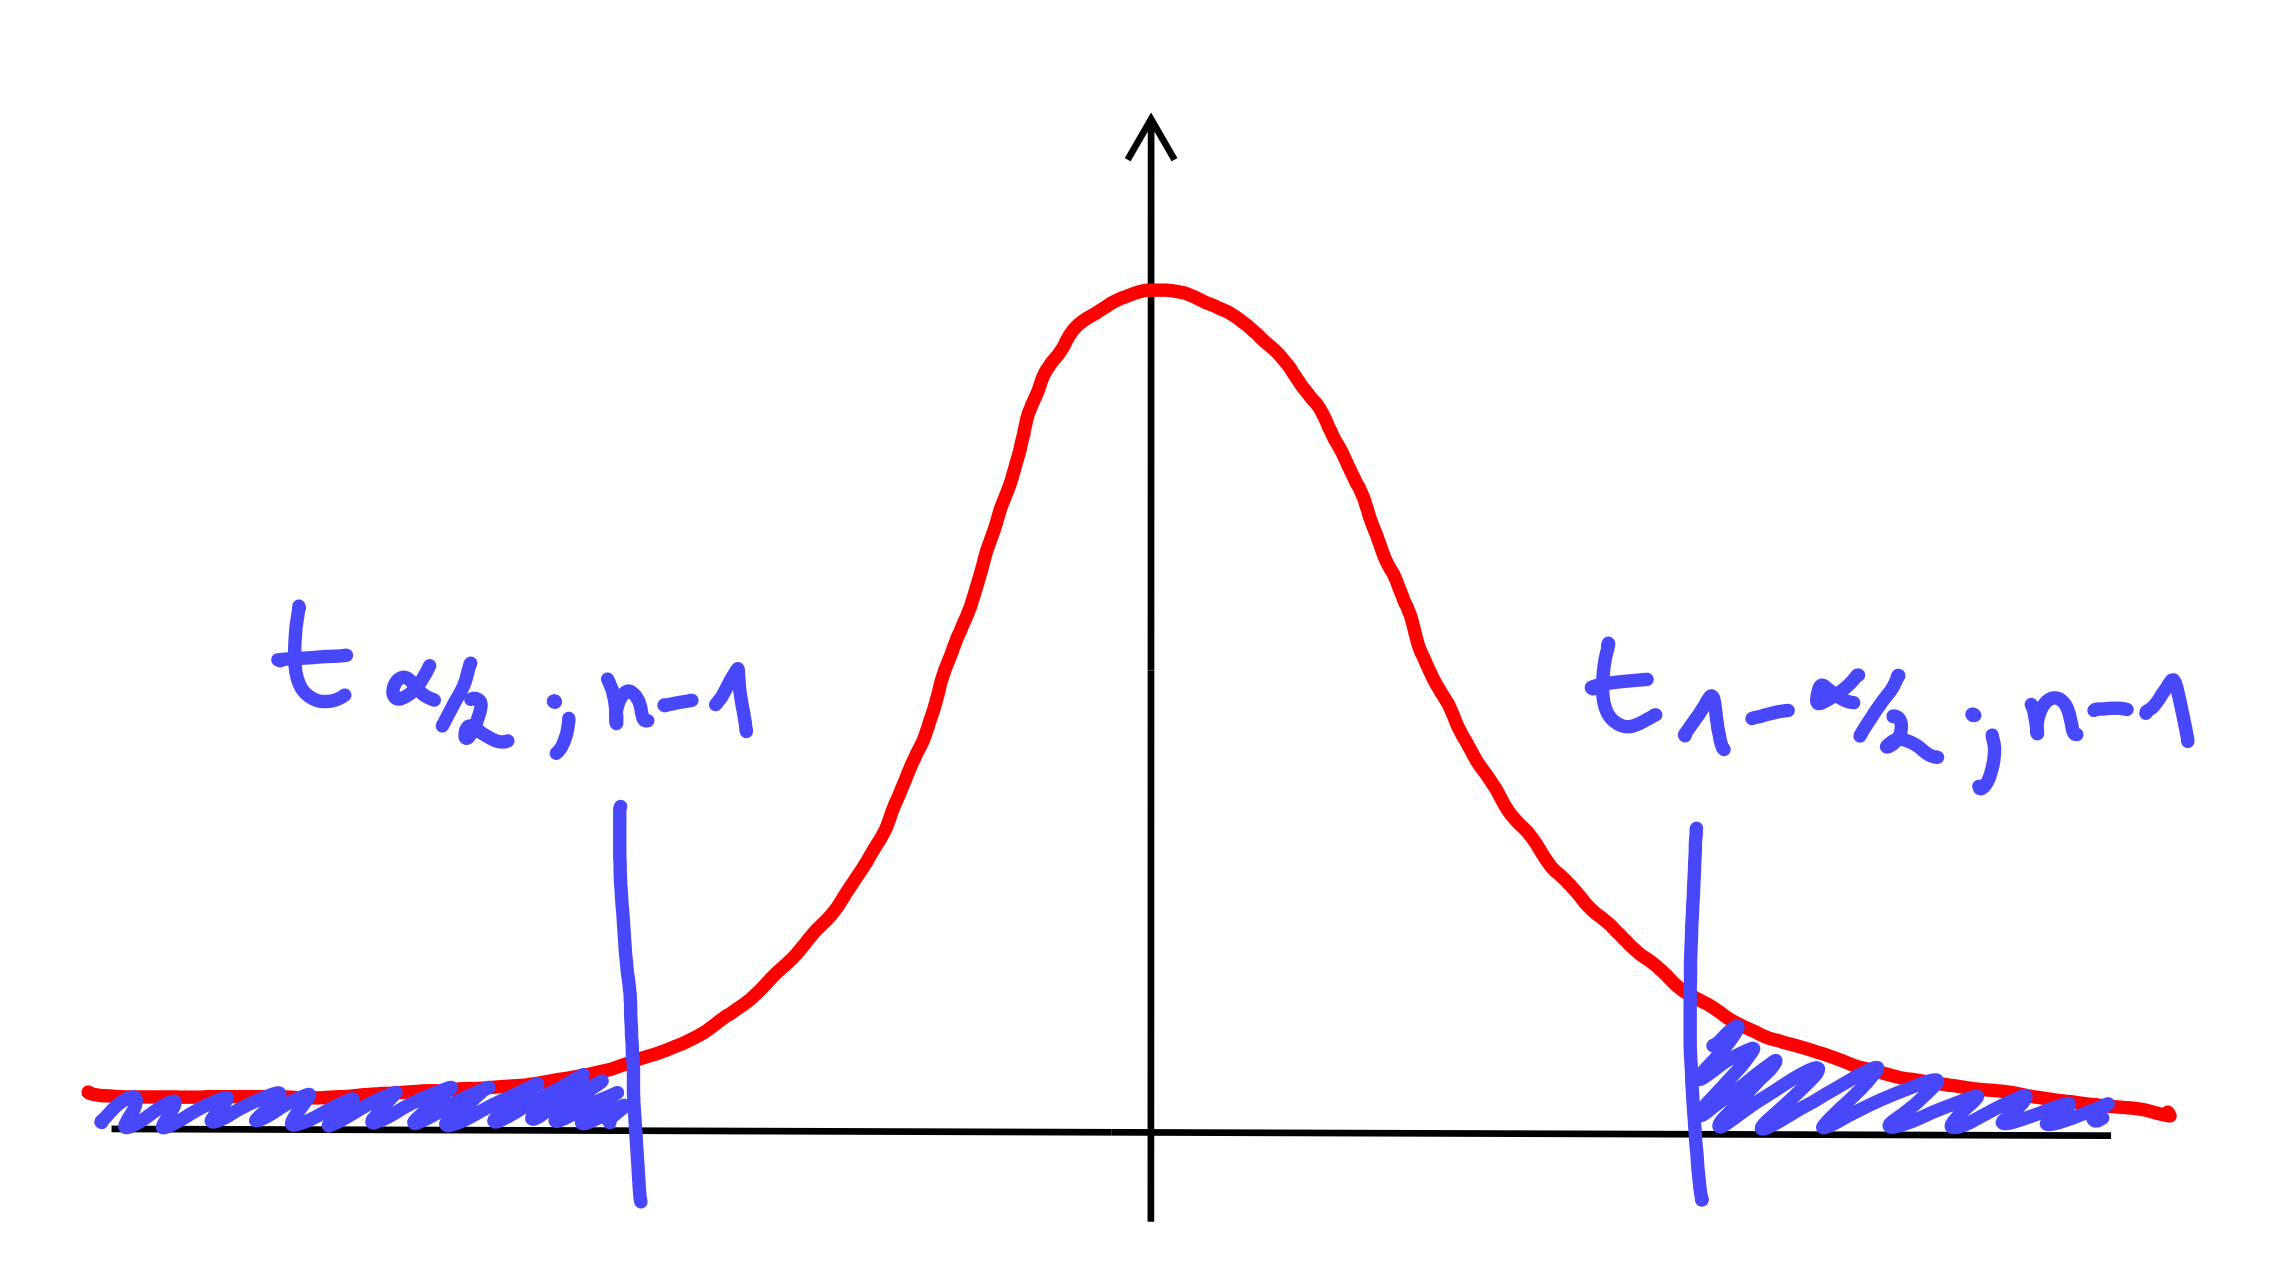
\includegraphics[scale=0.4]{5.png}
\end{center}
\end{frame}

\begin{frame}
\begin{itemize}
\item[b)] $H_0:\mu\geq\mu_0,~H_1:\mu< \mu_0$ \hfill $T=\frac{\bar{X}-\mu_0}{S}\sqrt{n}\sim t_{n-1}$ \hfill
\end{itemize}
\begin{center}
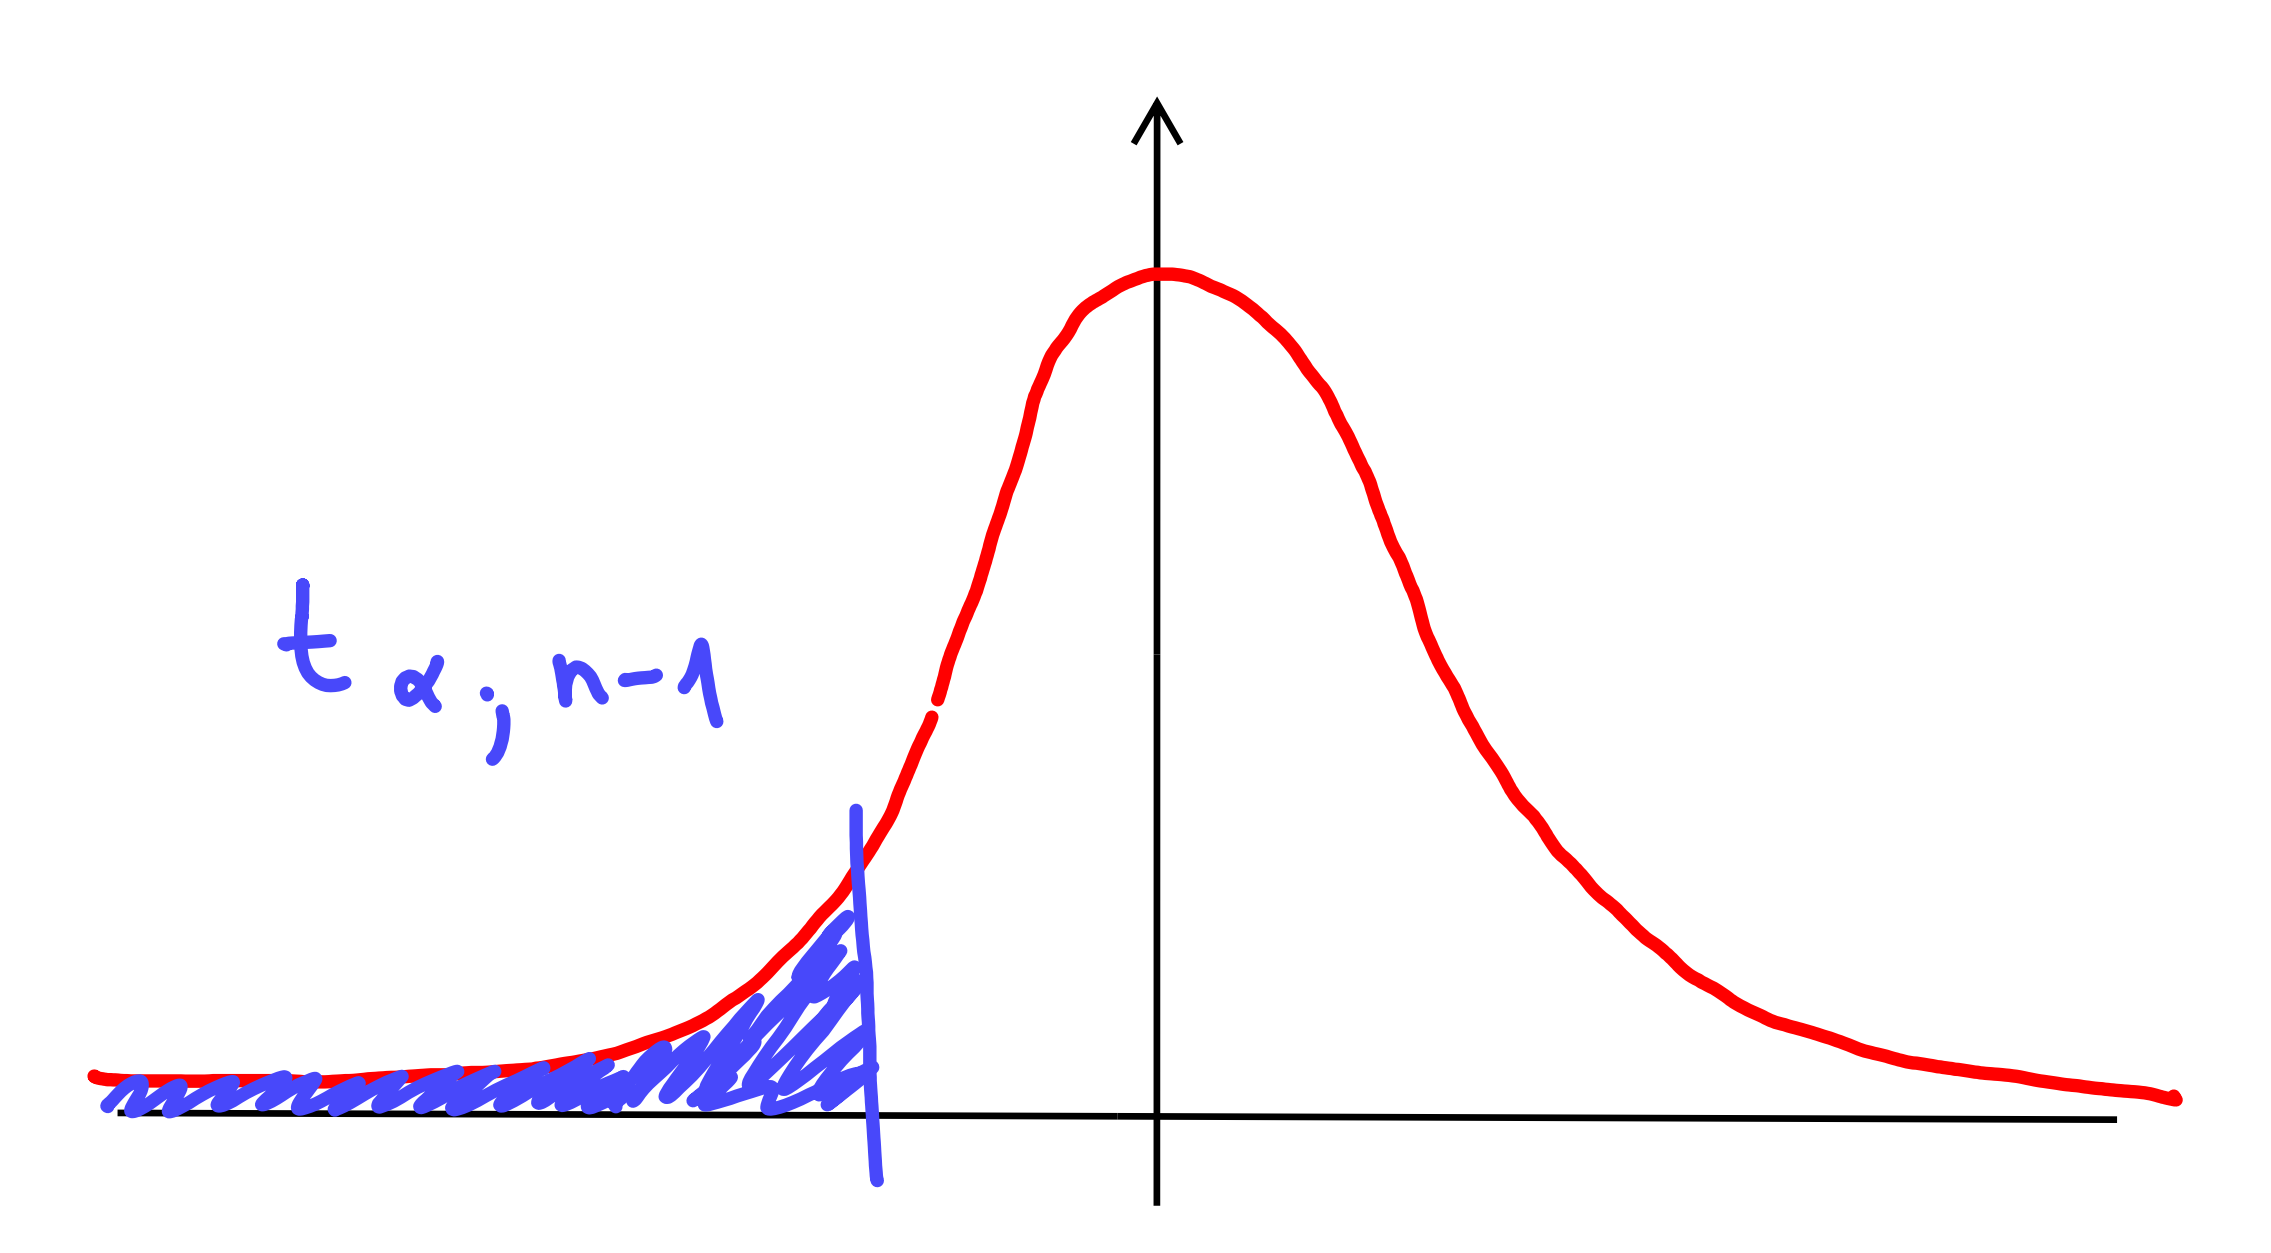
\includegraphics[scale=0.4]{6.png}
\end{center}
\end{frame}

\begin{frame}
\begin{itemize}
\item[c)] $H_0:\mu\leq\mu_0,~H_1:\mu > \mu_0$ \hfill $T=\frac{\bar{X}-\mu_0}{S}\sqrt{n}\sim t_{n-1}$ \hfill
\end{itemize}
\begin{center}
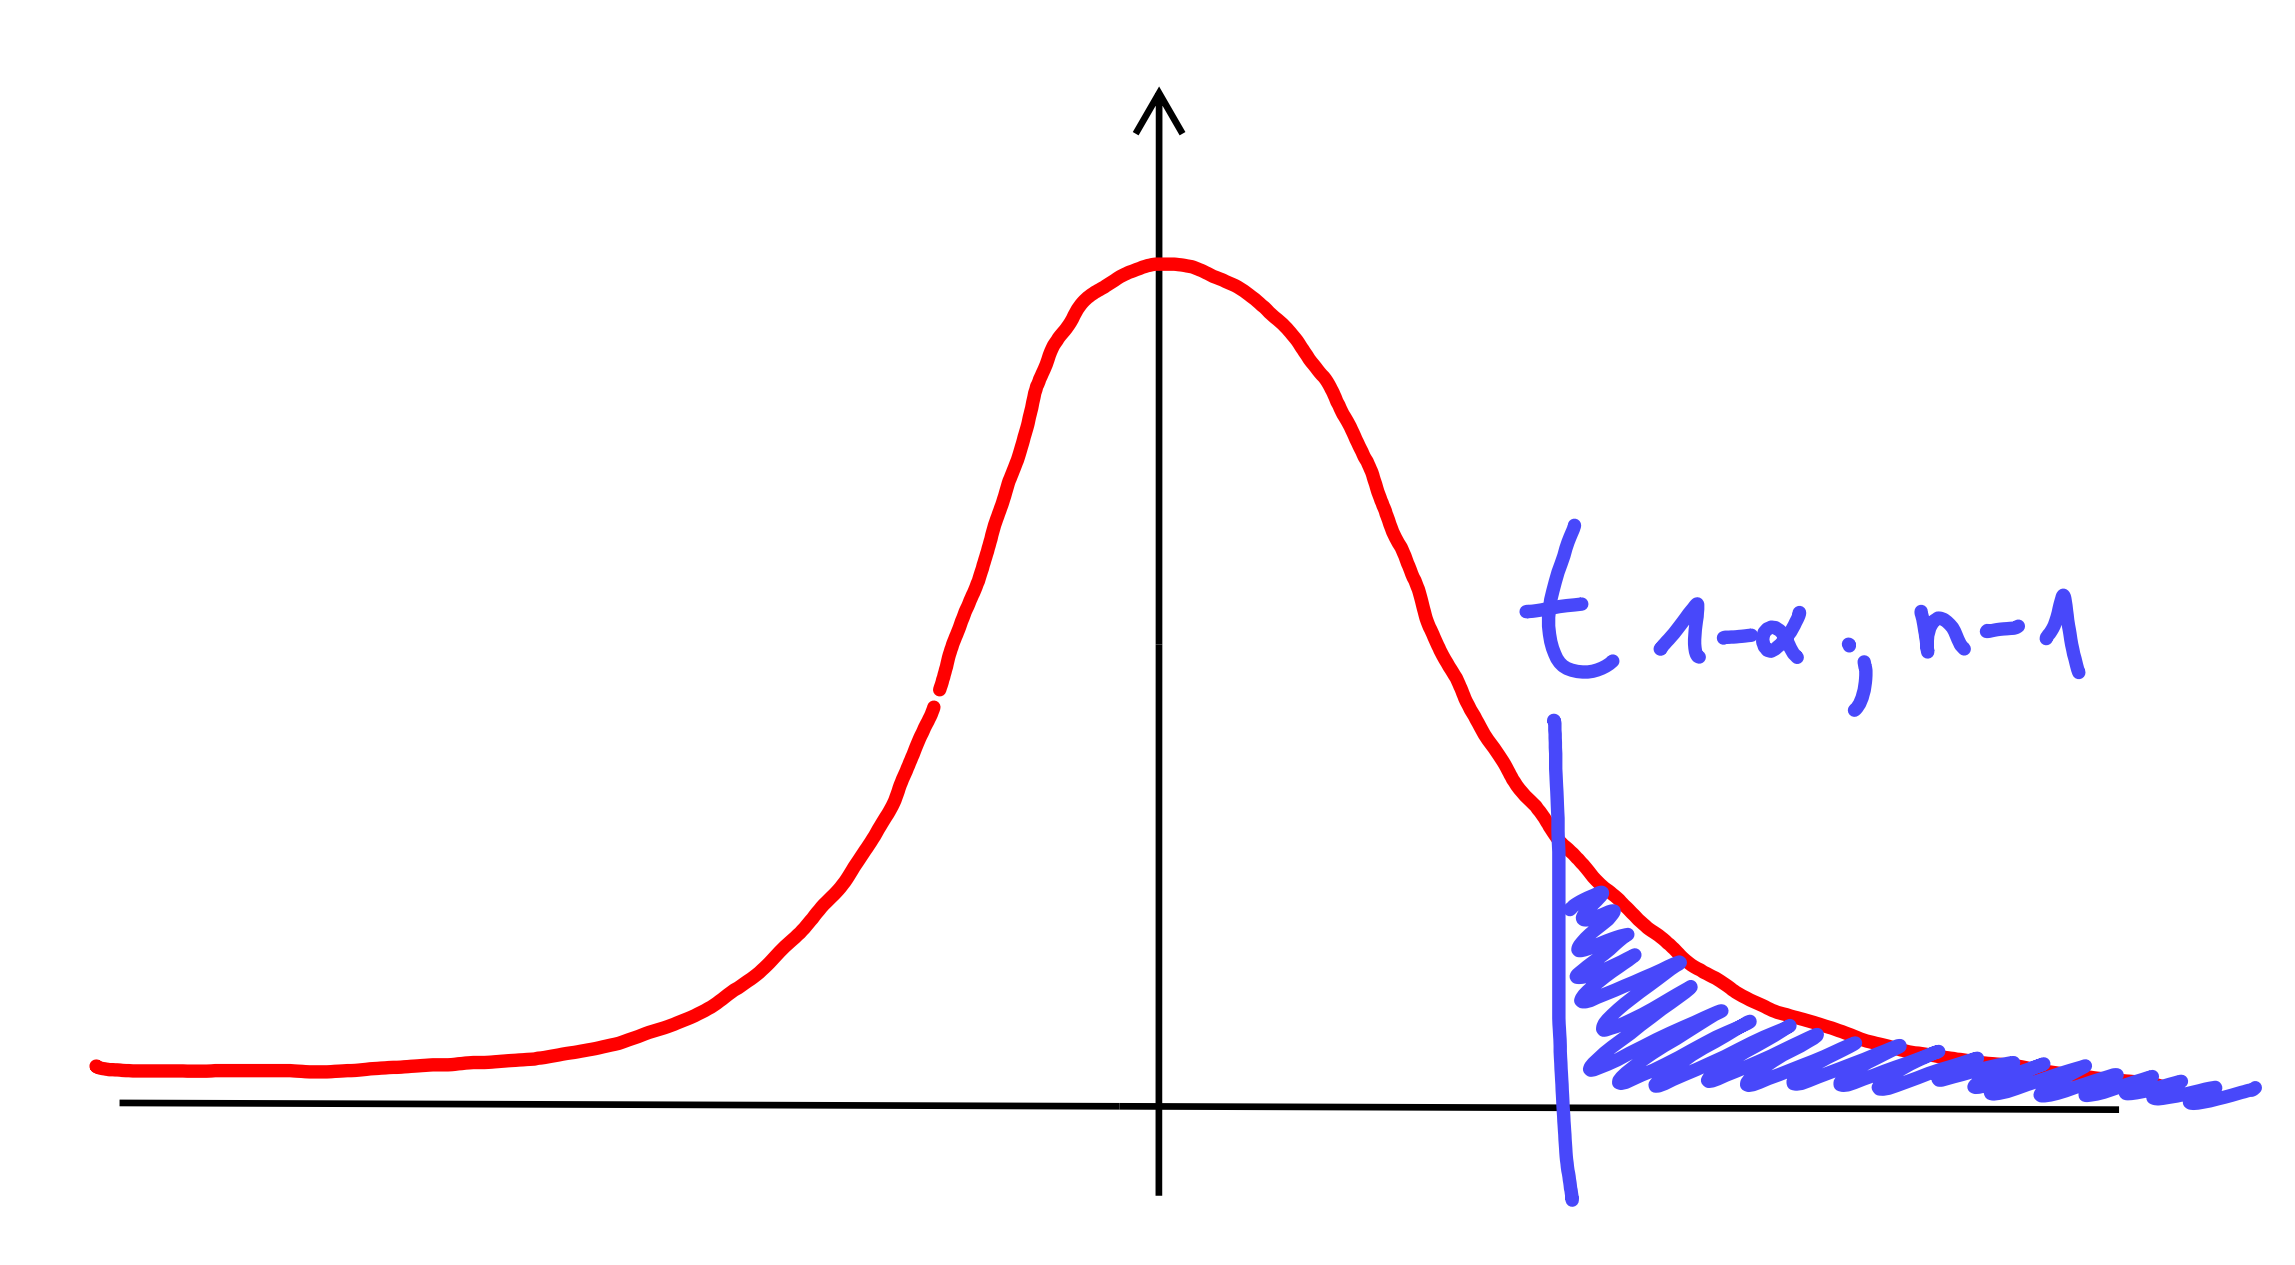
\includegraphics[scale=0.4]{7.png}
\end{center}
\end{frame}

\begin{frame}
\begin{block}{Beispiel}
	Eine Maschine soll automatisch 60 Gramm Müsli abwiegen und verpacken. Kleine Abweichungen sind dabei möglich, wir nehmen daher an, dass die abgepackte Menge normalverteilt ist. Wir überprüfen eine Stichprobe von 10 Verpackungen mit folgenden Mengen an Müsli (in Gramm):
	\begin{center}
		59.75 61.37 59.33 64.19 61.66 59.36 61.97 62.48 62.15 60.39
	\end{center}   
	Sind die Abweichungen von der Soll-Menge Zufall? Oder misst die Maschine nicht mehr auf 60 Gramm? Teste zu einem Konfidenzniveau von 95\%.
\end{block}
\end{frame}

\begin{frame}
Ausgangssituation:
$$ X_1,\dots,X_n\sim \mathcal{N}(\mu,\sigma^2)\text{~iid} $$

Hypothesen:
$$H_0:\mu=\mu_0,~H_1:\mu\neq\mu_0$$

Teststatistik:
$$ T=\frac{\bar{X}-\mu_0}{S}\sqrt{n} \sim t_{n-1} $$
\begin{center}
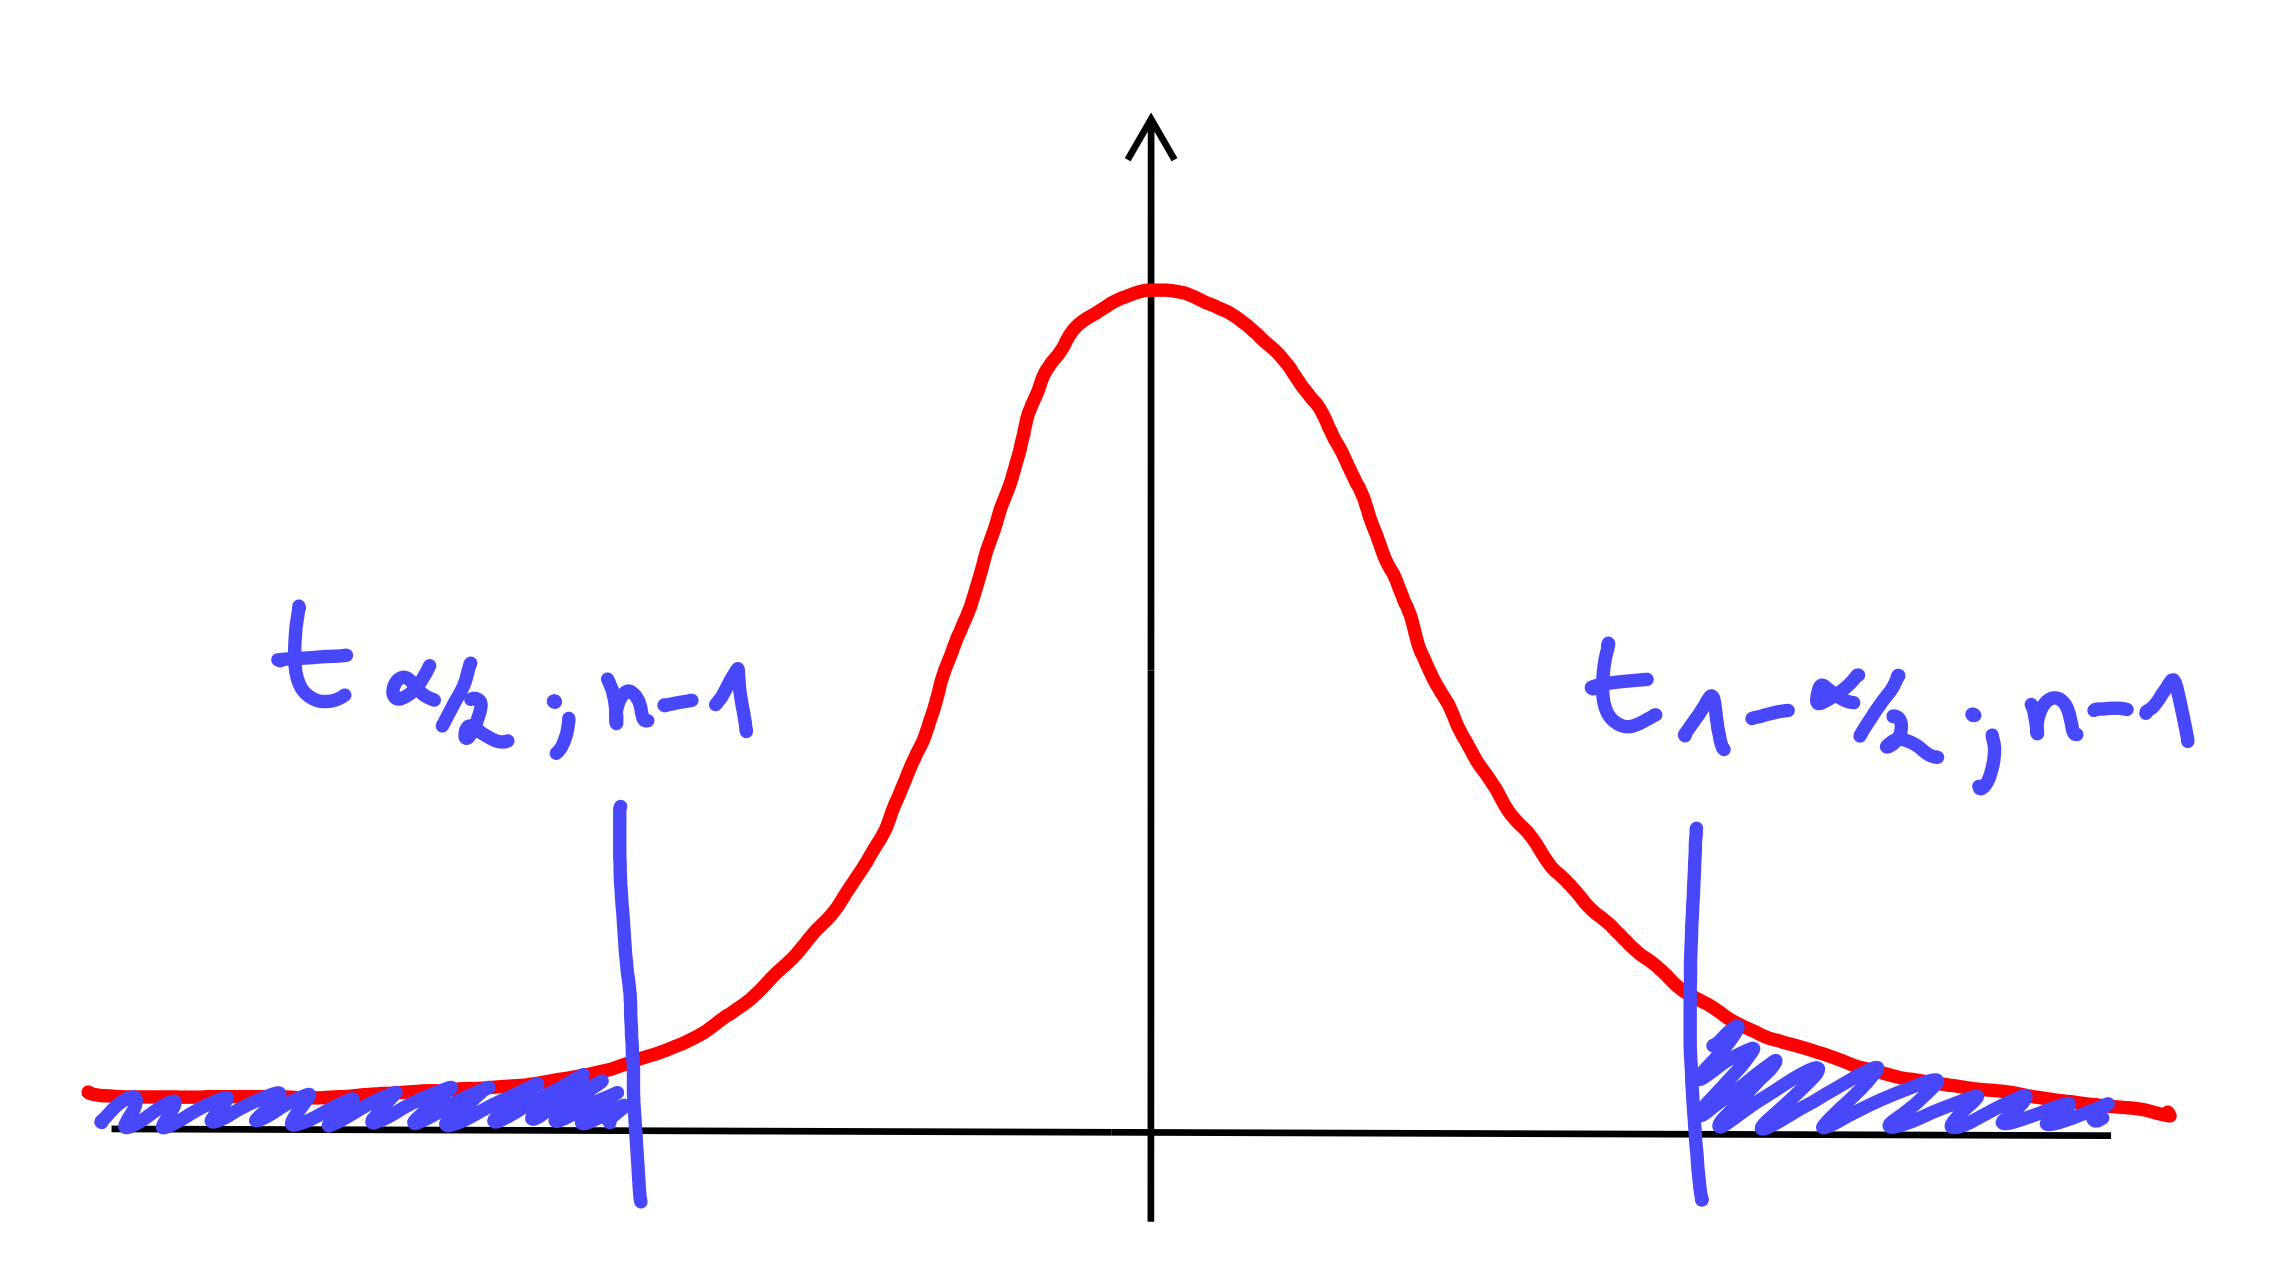
\includegraphics[scale=0.2]{5.png}
\end{center}
\end{frame}

\begin{frame}
Ausgangssituation:
$$ X_1,\dots,X_{10}\sim \mathcal{N}(\mu,\sigma^2)\text{~iid} $$

Hypothesen:
$$H_0:\mu=60,~H_1:\mu\neq 60$$

Teststatistik:
$$ T=\frac{\bar{X}-60}{S}\sqrt{10} \sim t_{9} $$
\begin{center}
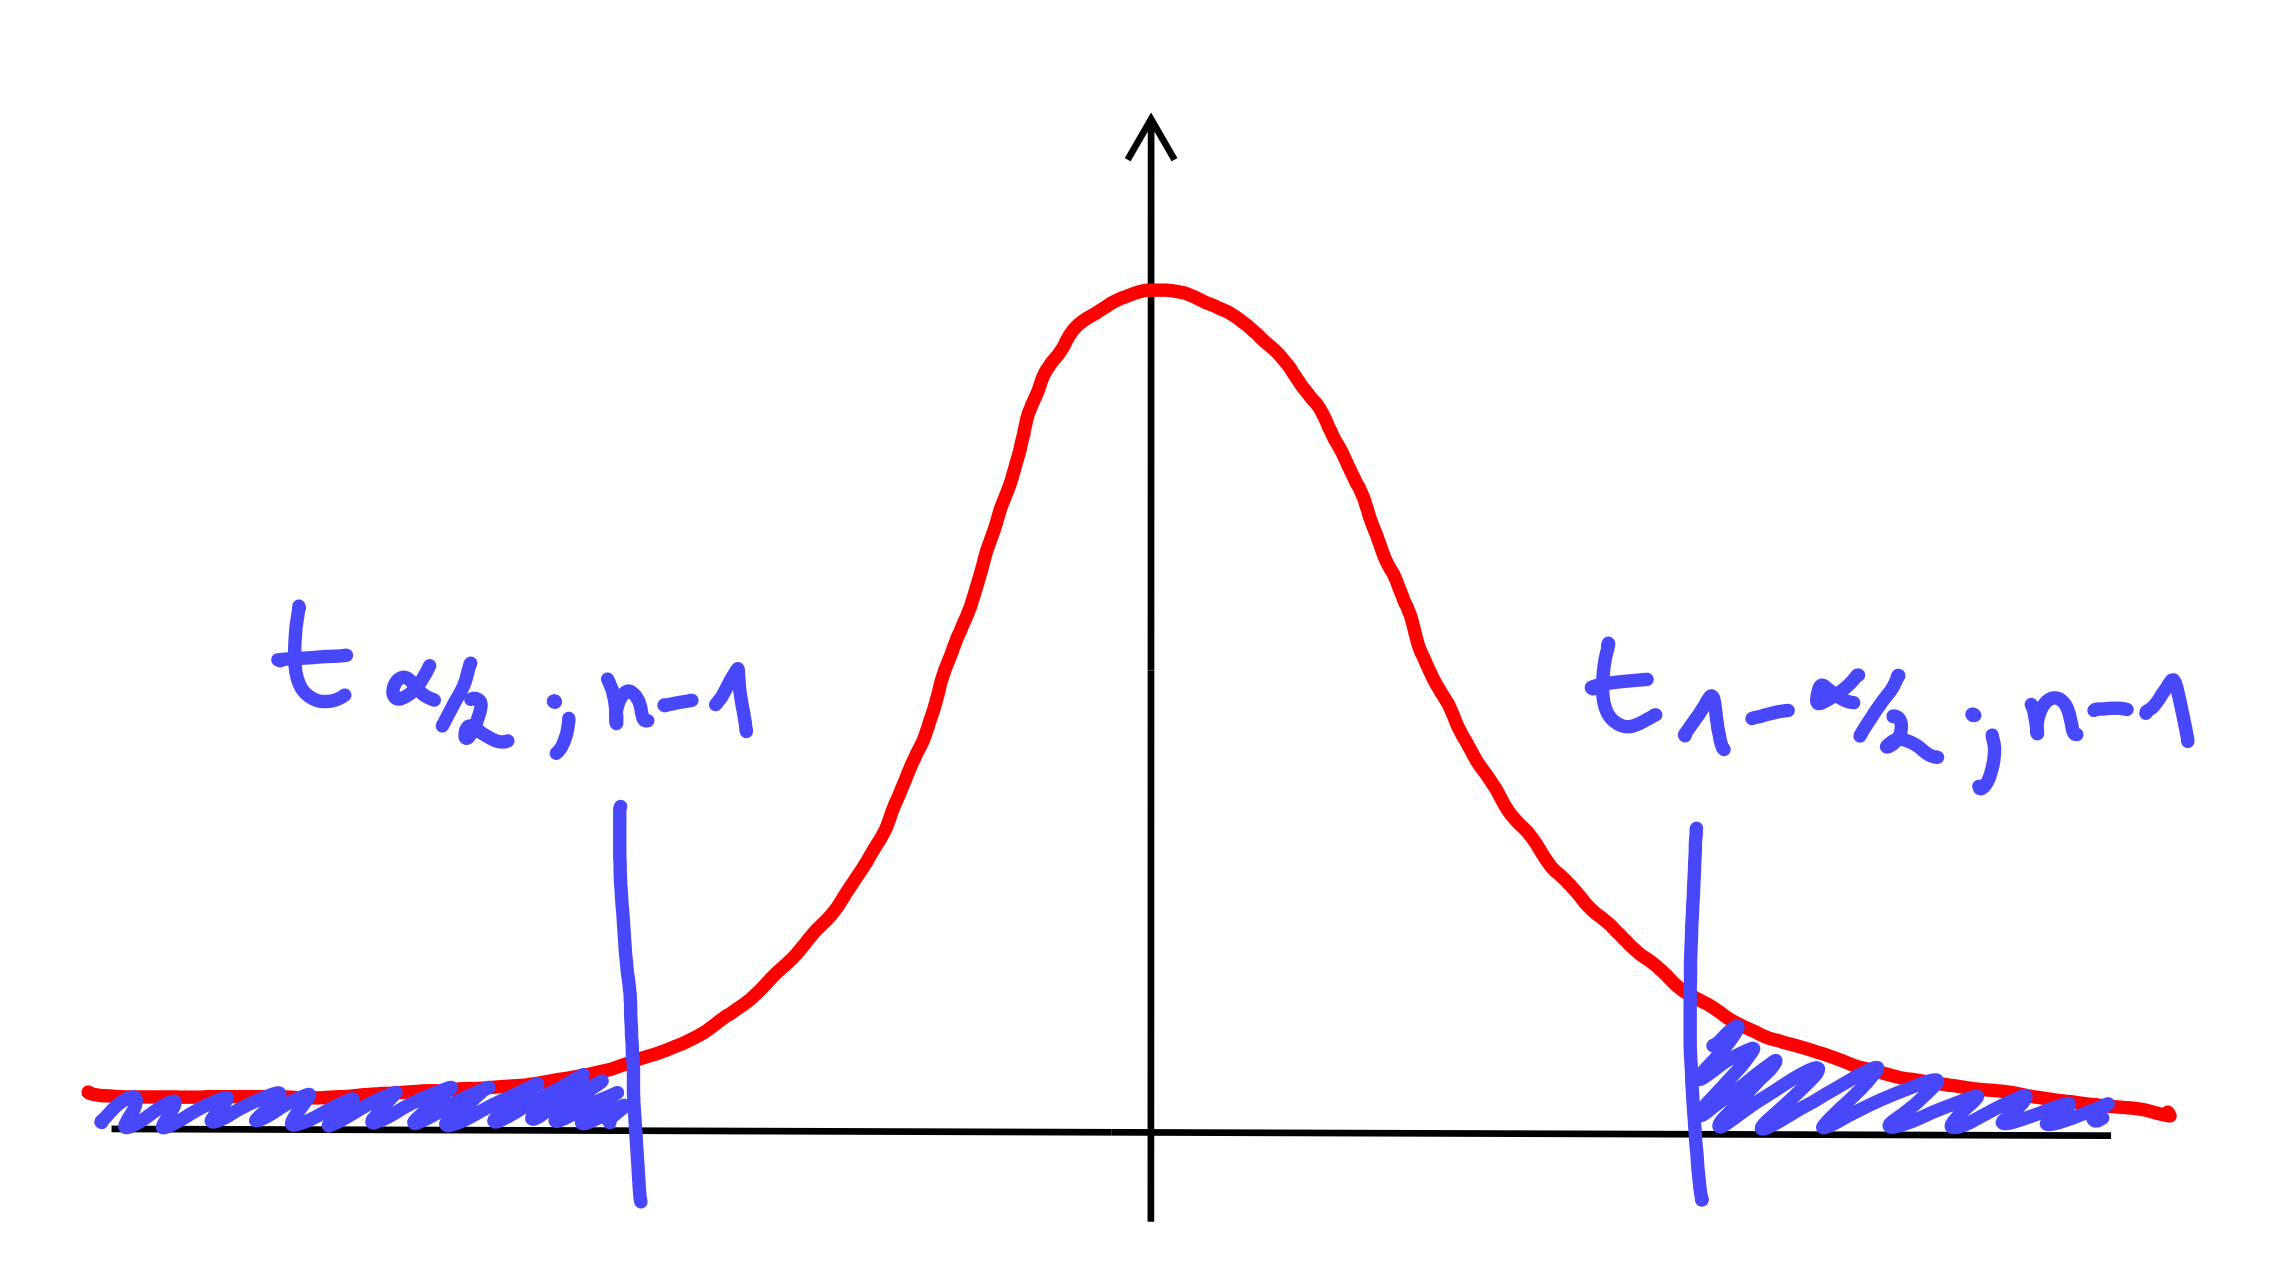
\includegraphics[scale=0.2]{5.png}
\end{center}
\end{frame}

\begin{frame}
$$ T=\frac{\bar{X}-60}{S}\sqrt{10} \sim t_{9} $$
\begin{center}
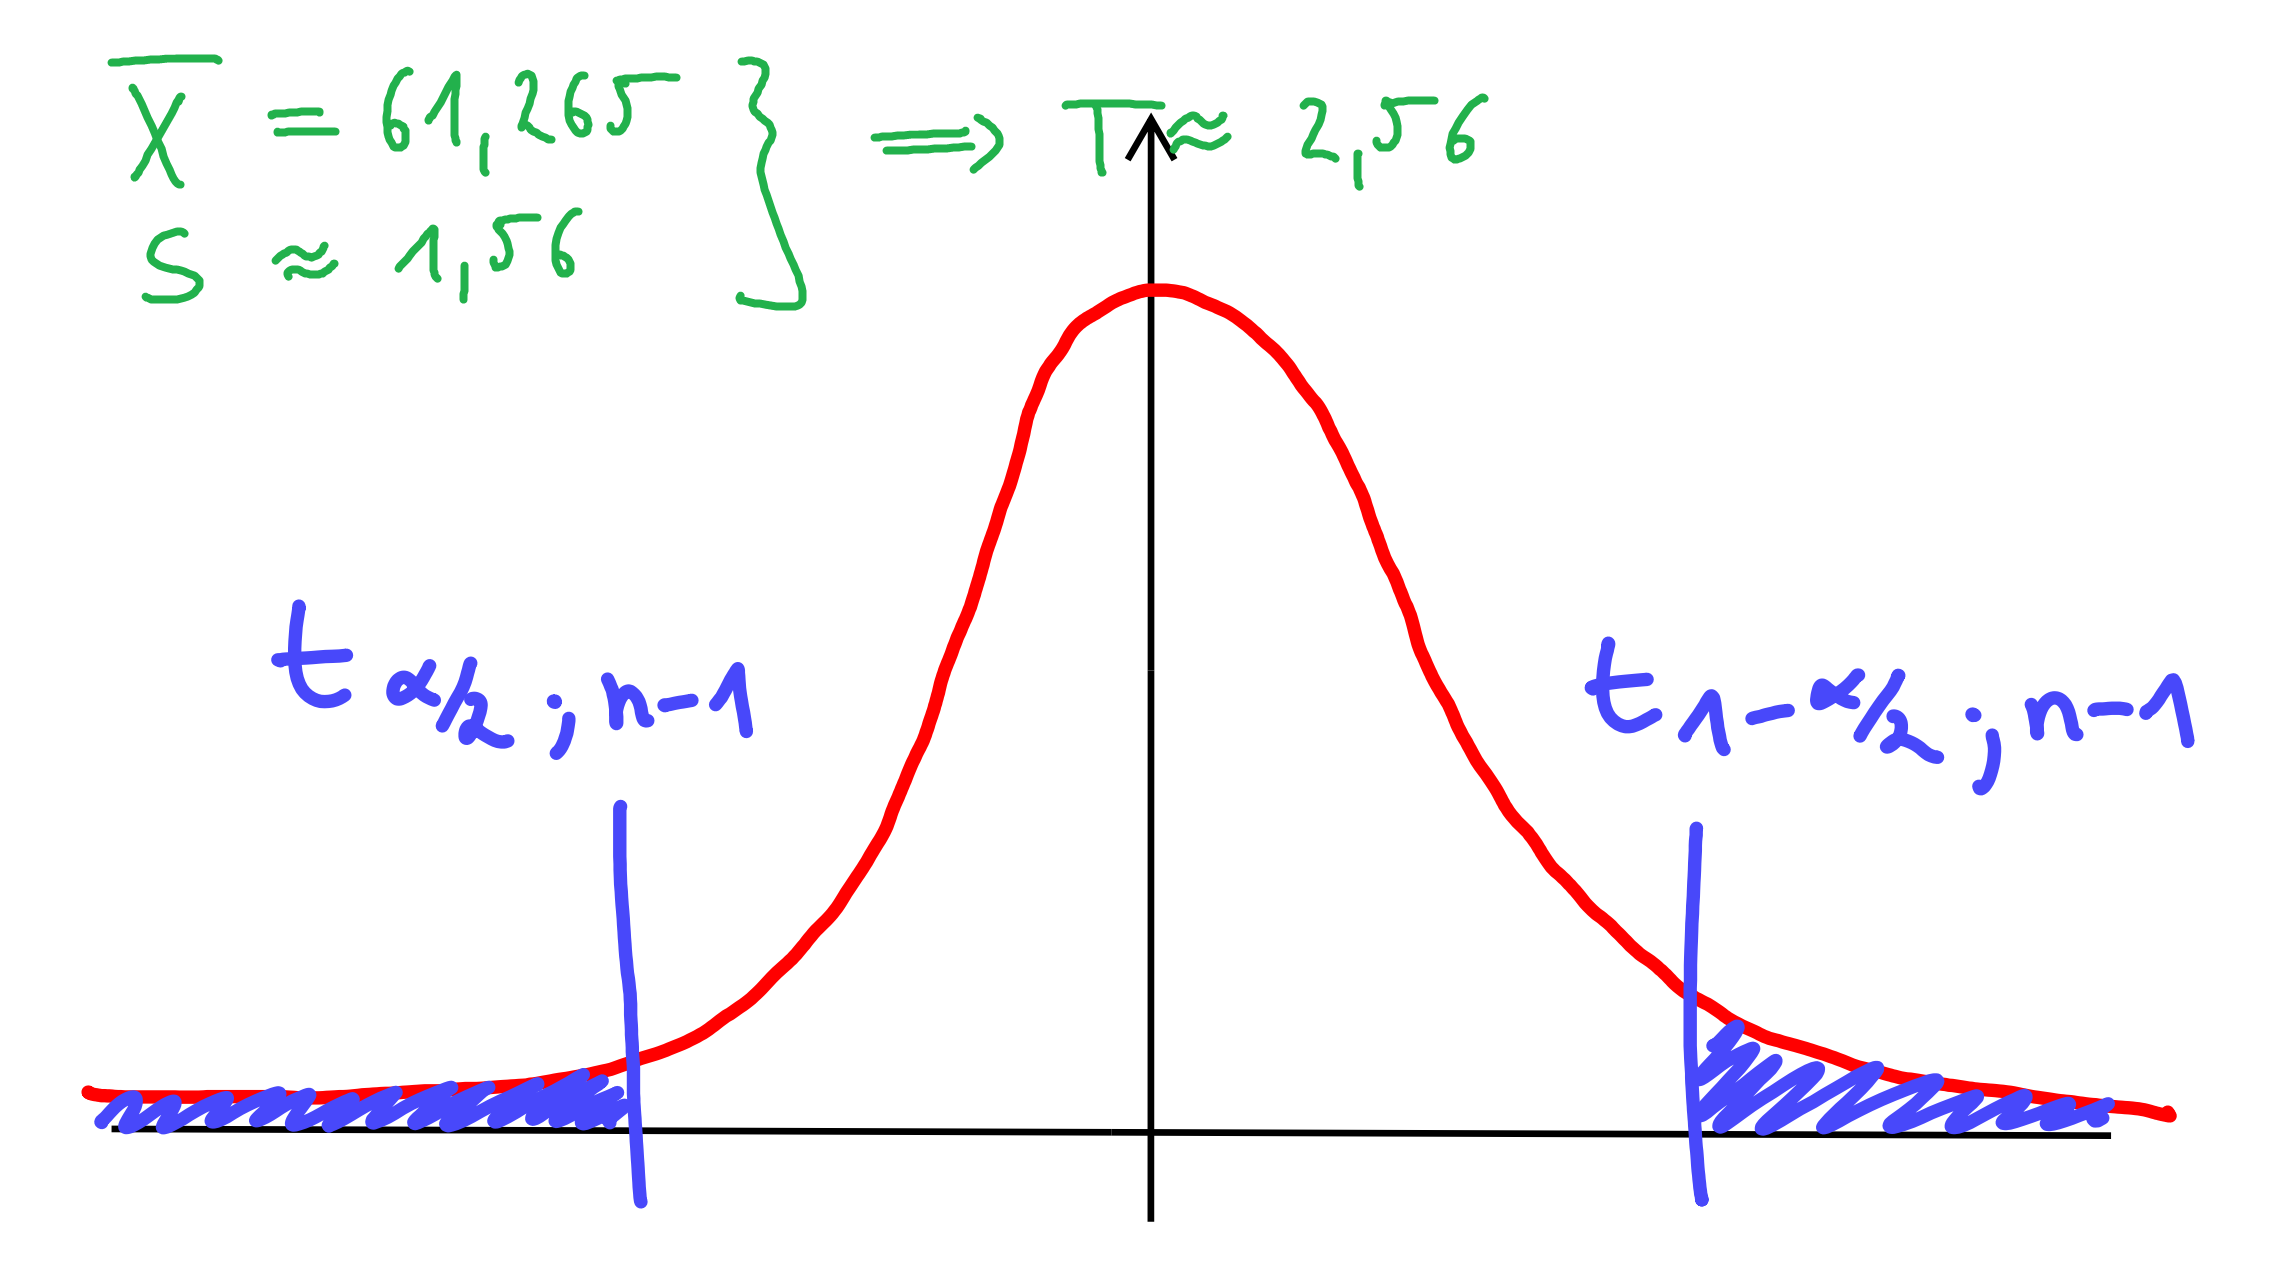
\includegraphics[scale=0.4]{5b.png}
\end{center}
\end{frame}

\begin{frame}
$$ T=\frac{\bar{X}-60}{S}\sqrt{10} \sim t_{9} $$
\begin{center}
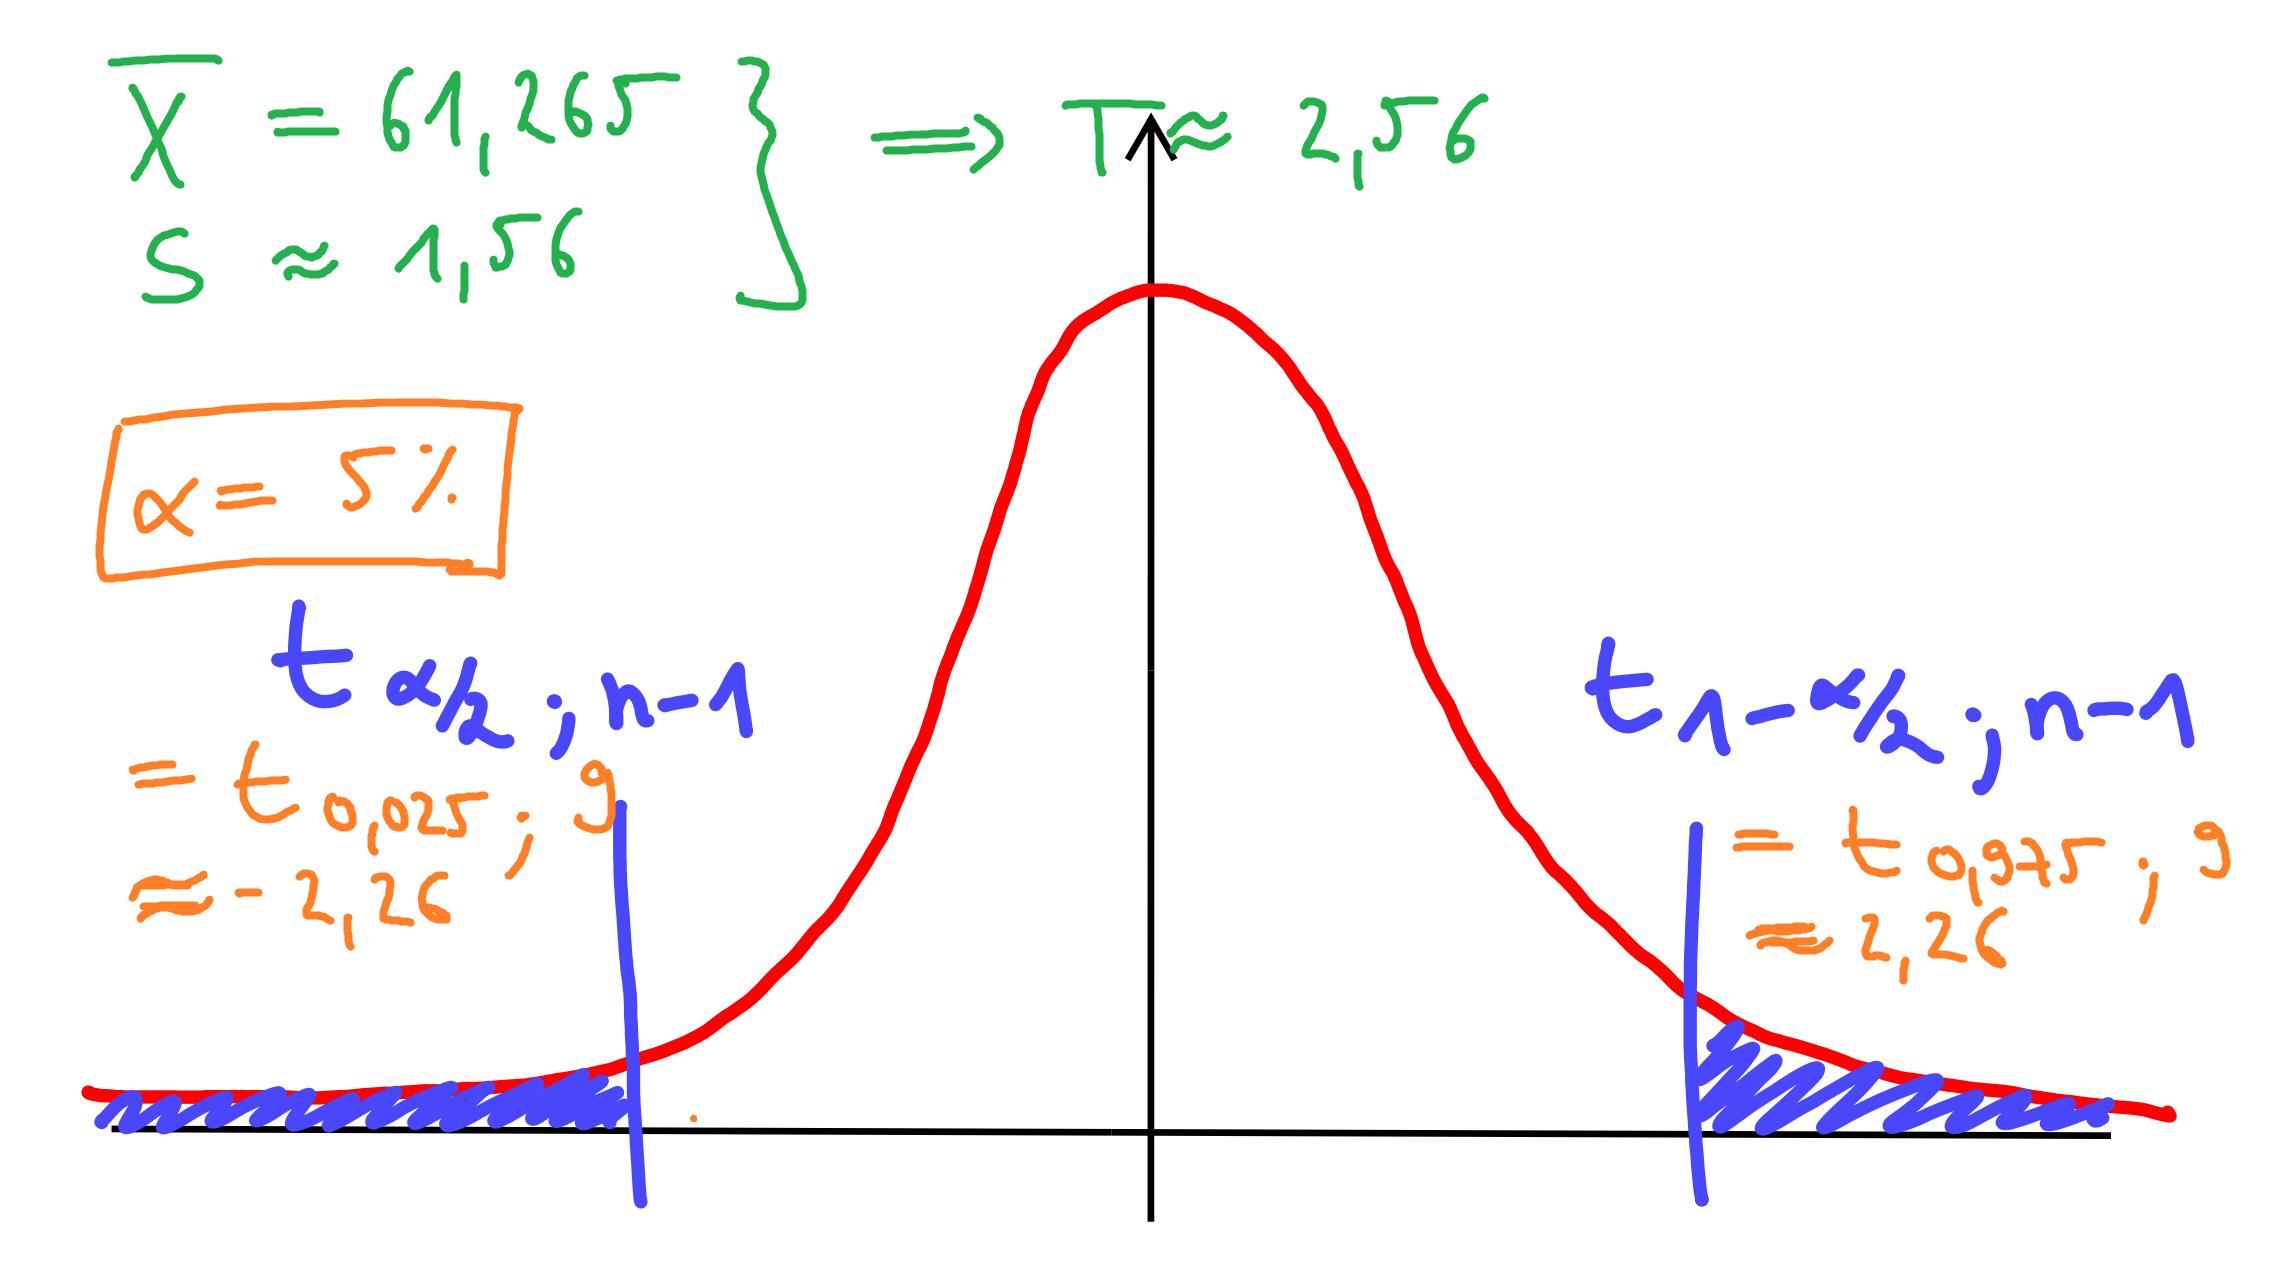
\includegraphics[scale=0.4]{5c.png}
\end{center}
\end{frame}

\begin{frame}
$$ T=\frac{\bar{X}-60}{S}\sqrt{10} \sim t_{9} $$
\begin{center}
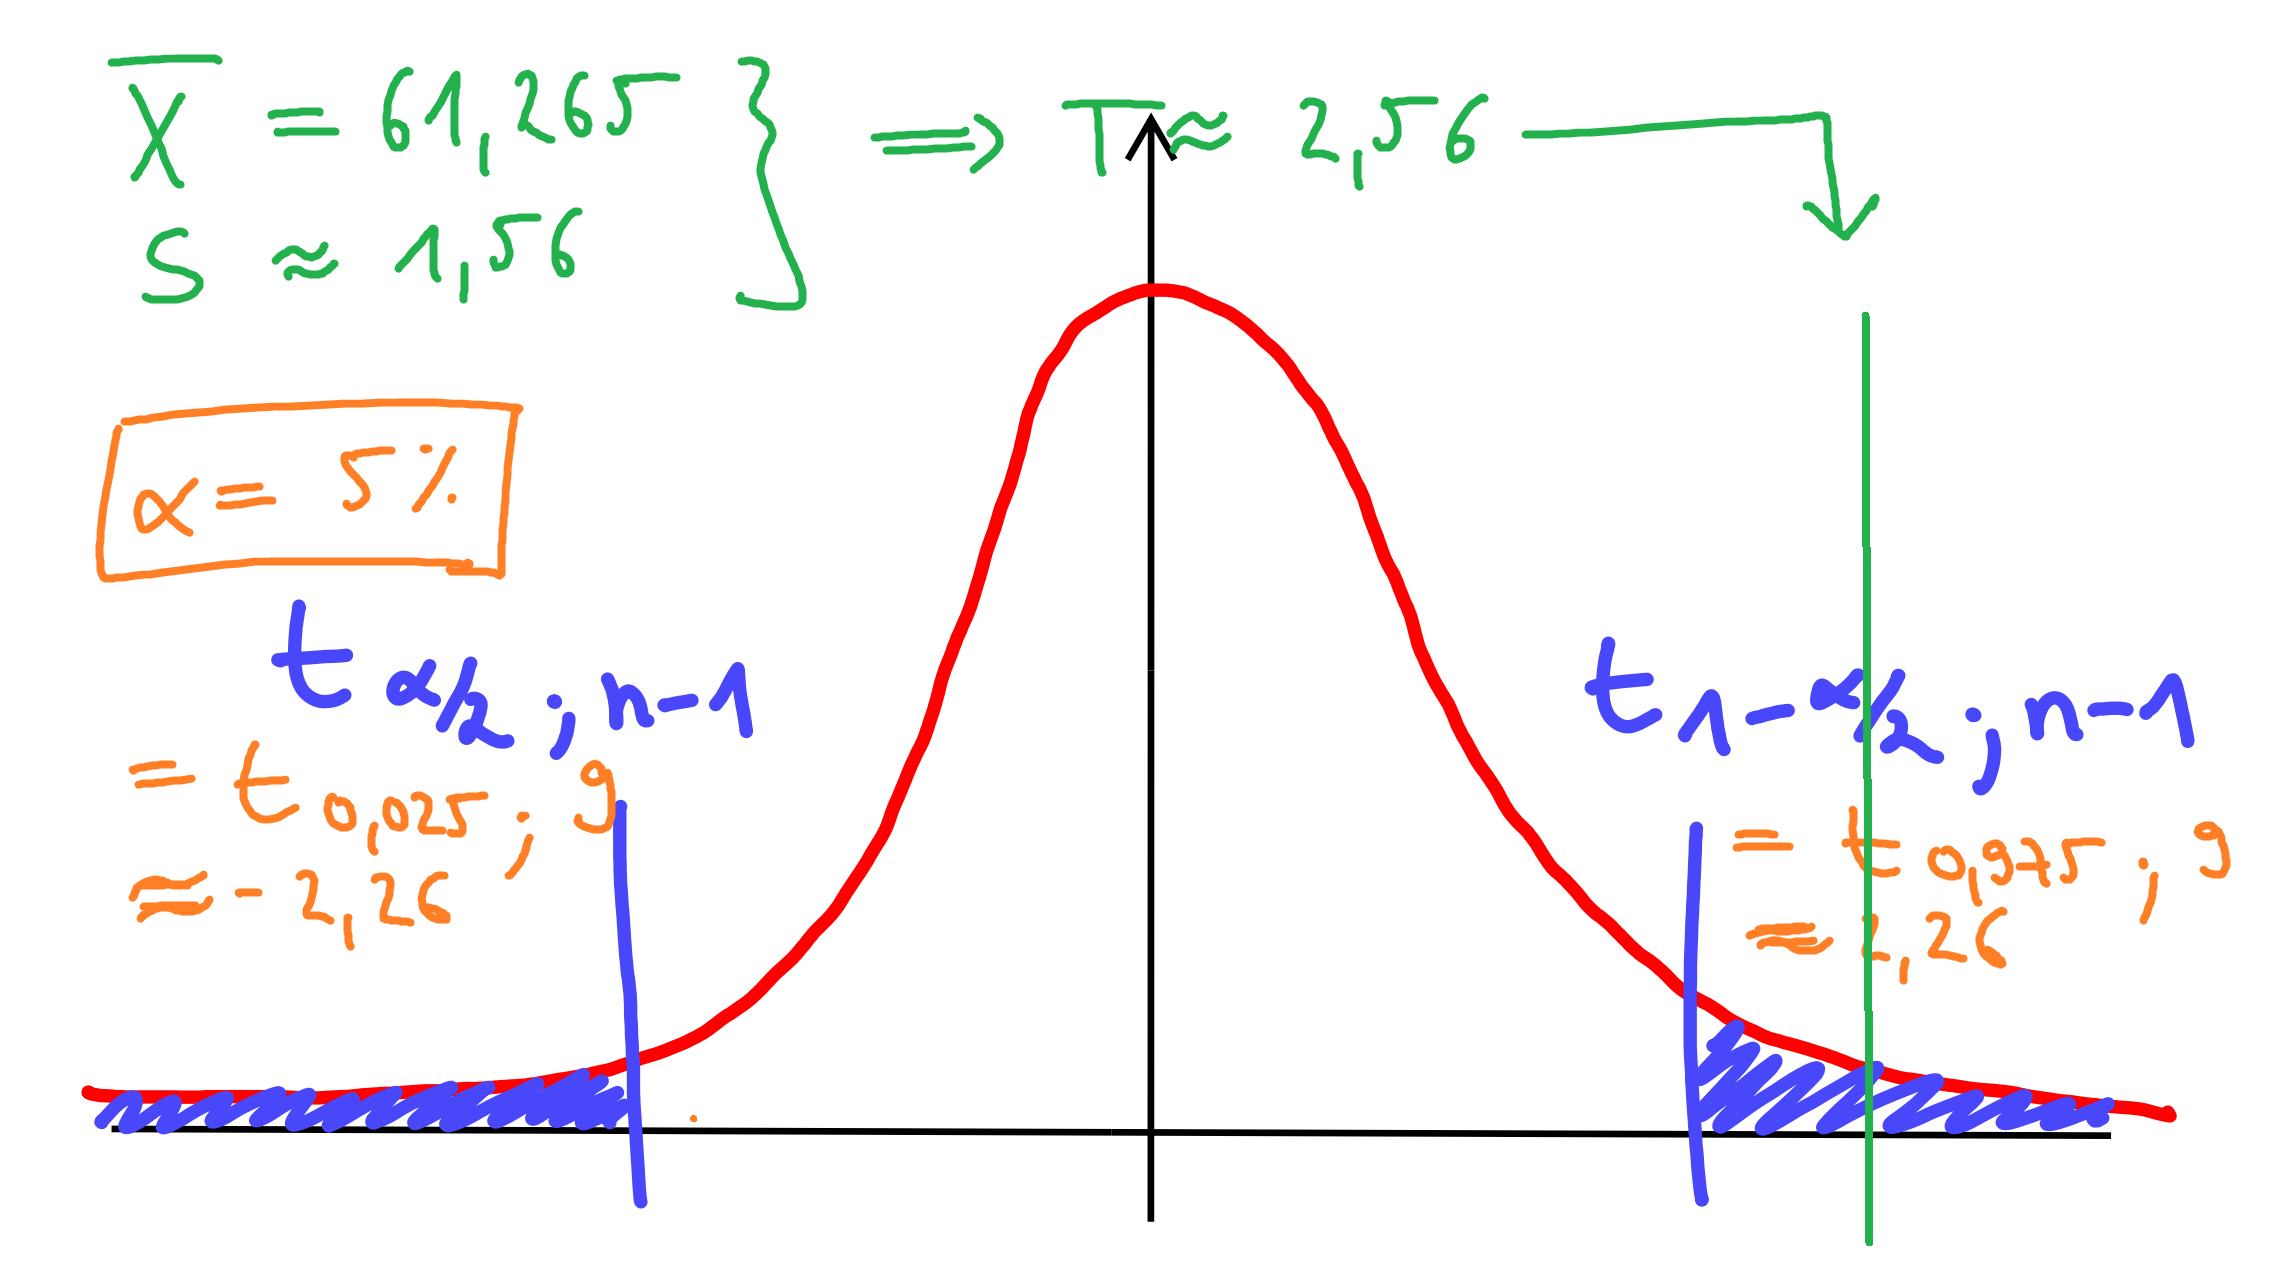
\includegraphics[scale=0.4]{5d.png}
\end{center}
\end{frame}

\end{document}